% ---------------------------------------------------------------------------------------------------------------
% TEMPLATE PARA TRABALHO DE CONCLUSÃO DE CURSO
% Universidade Tecnológica Federal do Paraná - UTFPR
% Customização da classe abnTeX2 (http://www.abntex.net.br/) para as normas da UTFPR
%
% Projeto hospedado em: <link git>
% Autores: Diego Marczal  <>
% 	   Michael Vornes <https://github.com/mvornes>
%
%----------------------------------------------------------------------------------------------------------------
% Codificação: UTF-8
% LaTeX:  abnTeX2          
% ---------------------------------------------------------------------------------------------------------------


% CARREGA CLASSE PERSONALIZADA DA UTFPR--------------------------------------------------------------------------
\documentclass[%twoside,                   % Impressão em frente e verso
    	        oneside,                   % Impressão apenas frente
]{configuracoes/utfpr-abntex2}


% INCLUI ARQUIVOS DE CONFIGURAÇÕES-------------------------------------------------------------------------------
% REFERÊNCIAS------------------------------------------------------------------
\usepackage[%
    alf,
    abnt-emphasize=bf,
    bibjustif,
    recuo=0cm,
    abnt-url-package=url,       % Utiliza o pacote url
    abnt-refinfo=yes,           % Utiliza o estilo bibliográfico abnt-refinfo
    abnt-etal-cite=3,
    abnt-etal-list=3,
    abnt-thesis-year=final
]{abntex2cite}                  % Configura as citações bibliográficas conforme a norma ABNT

% PACOTES----------------------------------------------------------------------
\usepackage[utf8]{inputenc}                                 % Codificação do documento
\usepackage[T1]{fontenc}                                    % Seleção de código de fonte
\usepackage{booktabs}                                       % Réguas horizontais em tabelas
\usepackage{color, colortbl}                                % Controle das cores
\usepackage{float}                                          % Necessário para tabelas/figuras em ambiente multi-colunas
\usepackage{graphicx}                                       % Inclusão de gráficos e figuras
\usepackage{icomma}                                         % Uso de vírgulas em expressões matemáticas
\usepackage{indentfirst}                                    % Indenta o primeiro parágrafo de cada seção
\usepackage{microtype}                                      % Melhora a justificação do documento
\usepackage{multirow, array}                                % Permite tabelas com múltiplas linhas e colunas
\usepackage{subeqnarray}                                    % Permite subnumeração de equações
\usepackage{lastpage}                                       % Para encontrar última página do documento
\usepackage{verbatim}                                       % Permite apresentar texto tal como escrito no documento, ainda que sejam comandos Latex
\usepackage{amsfonts, amssymb, amsmath}                     % Fontes e símbolos matemáticos
\usepackage[algoruled, portuguese]{algorithm2e}             % Permite escrever algoritmos em português
%\usepackage[scaled]{helvet}                                % Usa a fonte Helvetica
\usepackage{times}                                          % Usa a fonte Times
%\usepackage{palatino}                                      % Usa a fonte Palatino
%\usepackage{lmodern}                                       % Usa a fonte Latin Modern
\usepackage[bottom]{footmisc}                               % Mantém as notas de rodapé sempre na mesma posição
\usepackage{ae, aecompl}                                    % Fontes de alta qualidade
\usepackage{latexsym}                                       % Símbolos matemáticos
\usepackage{lscape}                                         % Permite páginas em modo "paisagem"
\usepackage{mathrsfs}
%\usepackage{picinpar}                                      % Dispor imagens em parágrafos
%\usepackage{scalefnt}                                      % Permite redimensionar tamanho da fonte
%\usepackage{subfig}                                        % Posicionamento de figuras
%\usepackage{upgreek}                                       % Fonte letras gregas

\newtheorem{mydef}{Definição}

% Redefine a fonte para uma fonte similar a Arial (fonte Helvetica)
\renewcommand*\familydefault{\sfdefault}

% CONFIGURAÇÕES DE APARÊNCIA DO PDF FINAL--------------------------------------
\makeatletter
\hypersetup{%
    portuguese,
    colorlinks=true,   % true: "links" coloridos; false: "links" em caixas de texto
    linkcolor=blue,    % Define cor dos "links" internos
    citecolor=blue,    % Define cor dos "links" para as referências bibliográficas
    filecolor=blue,    % Define cor dos "links" para arquivos
    urlcolor=blue,     % Define a cor dos "hiperlinks"
    breaklinks=true,
    pdftitle={\@title},
    pdfauthor={\@author},
    pdfkeywords={abnt, latex, abntex, abntex2}
}
\makeatother

% ALTERA O ASPECTO DA COR AZUL--------------------------------------------------
\definecolor{blue}{RGB}{41,5,195}

% REDEFINIÇÃO DE LABELS---------------------------------------------------------
\renewcommand{\algorithmautorefname}{Algoritmo}
\def\equationautorefname~#1\null{Equa\c c\~ao~(#1)\null}

% CRIA ÍNDICE REMISSIVO---------------------------------------------------------
\makeindex

% HIFENIZAÇÃO DE PALAVRAS QUE NÃO ESTÃO NO DICIONÁRIO---------------------------
\hyphenation{%
    qua-dros-cha-ve
    Kat-sa-gge-los
}



% INCLUI ARQUIVOS DO TRABALHO DE CONCLUSÃO DE CURSO (PRÉ-TEXTUAIS, TEXTUAIS, PÓS-TEXTUAIS)-----------------------

% INSERE CAPA E FOLHA DE ROSTO
% CAPA---------------------------------------------------------------------------------------------------

% ORIENTAÇÕES GERAIS-------------------------------------------------------------------------------------
% Caso algum dos campos não se aplique ao seu trabalho, como por exemplo,
% se não houve coorientador, apenas deixe vazio.
% Exemplos: 
% \coorientador{}
% \departamento{}

% DADOS DO TRABALHO--------------------------------------------------------------------------------------
\titulo{Consultas por similaridade em bases de dados complexos utilizando técnica OMNI em SGBDR}
\titleabstract{Similarity queries in complex databases using OMNI technique in RDBMS}
\autor{Cristiano José Mendes Matsui}
\autorcitacao{MATSUI, Cristiano} % Sobrenome em maiúsculo
\local{Pato Branco}
\data{2018}

% NATUREZA DO TRABALHO-----------------------------------------------------------------------------------
% Opções: 
% - Trabalho de Conclusão de Curso (se for Graduação)
% - Dissertação (se for Mestrado)
% - Tese (se for Doutorado)
% - Projeto de Qualificação (se for Mestrado ou Doutorado)
\projeto{Trabalho de Conclusão de Curso}

% TÍTULO ACADÊMICO---------------------------------------------------------------------------------------
% Opções:
% - Bacharel ou Tecnólogo (Se a natureza for Trabalho de Conclusão de Curso)
% - Mestre (Se a natureza for Dissertação)
% - Doutor (Se a natureza for Tese)
% - Mestre ou Doutor (Se a natureza for Projeto de Qualificação)
\tituloAcademico{Bacharel}

% ÁREA DE CONCENTRAÇÃO E LINHA DE PESQUISA---------------------------------------------------------------
% Se a natureza for Trabalho de Conclusão de Curso, deixe ambos os campos vazios
% Se for programa de Pós-graduação, indique a área de concentração e a linha de pesquisa
\areaconcentracao{}
\linhapesquisa{}

% DADOS DA INSTITUIÇÃO-----------------------------------------------------------------------------------
% Se a natureza for Trabalho de Conclusão de Curso, coloque o nome do curso de graduação em "programa"
% Formato para o logo da Instituição: \logoinstituicao{<escala>}{<caminho/nome do arquivo>}
\instituicao{Universidade Tecnológica Federal do Paraná}
\departamento{DAINF - Departamento Acadêmico de Informática}
\programa{Curso de Engenharia de Computação}
\logoinstituicao{0.2}{dados/figuras/logo-instituicao.png} 

% DADOS DOS ORIENTADORES---------------------------------------------------------------------------------

%\orientador[Orientadora:]{Nome da orientadora}
\orientador{Dr. Ives Renê Venturini Pola}
\coorientador[Coorientadora:]{Dra. Fernanda Paula Barbosa Pola}
%\coorientador[Coorientadora:]{Nome da coorientadora}


% FOLHA DE ROSTO--------------------------------------------------------------------------------------------------------

% TRABALHO DE CONCLUSÃO DE CURSO
 \preambulo{{\imprimirprojeto} de graduação, apresentado à disciplina de Trabalho de Conclusão de Curso 1, do {\imprimirprograma} - TSI - da {\imprimirinstituicao} - UTFPR - Câmpus Guarapuava, como requisito parcial para a obtenção do título de {\imprimirtituloAcademico} em Sistemas para Internet.}

% OBSERVAÇÕES-----------------------------------------------------------------------------------------------------------
% Este arquivo não precisa ser alterado.


\begin{document}

\pretextual
\imprimircapa                                               	           % Comando para imprimir Capa
\imprimirfolhaderosto{}                                     		   % Comando para imprimir Folha de rosto
% INSERE ELEMENTOS PRÉ-TEXTUAIS
% DEDICATÓRIA------------------------------------------------------------------

\renewcommand{\dedicatorianame}{DEDICATÓRIA}

\begin{dedicatoria}

Altere este texto inserindo a dedicatória do seu trabalho. 

\end{dedicatoria}
          			   % Dedicatória
% AGRADECIMENTOS---------------------------------------------------------------

\begin{agradecimentos}[AGRADECIMENTOS]

Edite e coloque aqui os agradecimentos às pessoas e/ou instituições que contribuíram para a realização do trabalho.

É obrigatório o agradecimento às instituições de fomento à pesquisa que financiaram total ou parcialmente o trabalho, inclusive no que diz respeito à concessão de bolsas.

\end{agradecimentos}
        			   % Agradecimentos
% EPÍGRAFE---------------------------------------------------------------------

\renewcommand{\epigraphname}{EPÍGRAFE}

\begin{epigrafe}

\textit{Eu denomino meu campo de Gestão do Conhecimento, mas você não pode gerenciar conhecimento. Ninguém pode. O que pode fazer - o que a empresa pode fazer - é gerenciar o ambiente que otimize o conhecimento. (PRUSAK, Laurence, 1997).}

\end{epigrafe}

% OBSERVAÇÕES------------------------------------------------------------------
% Altere o texto para inserir a epígrafe do seu trabalho

              			   % Epígrafe
% RESUMO--------------------------------------------------------------------------------

\begin{resumo}[RESUMO]
\begin{SingleSpacing}
    
% Não altere esta seção do texto--------------------%TODO ISSO AQUI É HARD CODED--------------------------
\imprimirautorcitacao. \imprimirtitulo. \imprimirdata. 26 f. \imprimirprojeto\ – \imprimirprograma, \imprimirinstituicao. \imprimirlocal, \imprimirdata.\\ 
%---------------------------------------------------------------------------------------
					
A necessidade de armazenamento de mídias cada vez maiores em termos de tamanho de armazenamento e complexas é uma tendência que aumentou consideravelmente
com os avanços da tecnologia e comunicação. Estes dados conhecidos como dados complexos exigem uma complexidade estrutural
de armazenamento e análise maior do que dados simples como palavras ou números, além de requererem operadores especiais
de consultas, como a consulta por abrangência (Rq) e a consulta aos k-vizinhos mais próximos (kNNq). Dentre o conjunto de dados complexos
destacam-se as imagens, que precisam ser comparadas de acordo com características extraídas como cor, forma ou textura. Esta
comparação é realizada na forma de um cálculo de distância entre o valor da característica da imagem central da consulta em relação
a todas as outras imagens da base de dados. O tempo de consulta pode aumentar significativamente com o aumento da base de dados. 
Para contornar o problema da maldição da cardinalidade, este trabalho tem como proposta aplicar uma técnica (Omni) utilizada para promover 
uma etapa de filtragem do número de imagens a terem as suas distâncias calculadas, evitando a comparação com toda a base de dados.
Após a modelagem e construção de um banco de dados que suporte esta técnica, será implementado um sistema de recuperação de imagens
(CBIR).\\

\textbf{Palavras-chave}: Dados Complexos. OMNI. CBIR. Rq. kNNq.

\end{SingleSpacing}
\end{resumo}

% OBSERVAÇÕES---------------------------------------------------------------------------
% Altere o texto inserindo o Resumo do seu trabalho.
% Escolha de 3 a 5 palavras ou termos que descrevam bem o seu trabalho 

%TODO PADRONIZAR TÉCNICAS OMNI/TÉCNICA OMNI             			   % Resumo em Português
% ABSTRACT--------------------------------------------------------------------------------

\begin{resumo}[ABSTRACT]
\begin{SingleSpacing}

% Não altere esta seção do texto--------------------------------------------------------
\imprimirautorcitacao. \imprimirtitleabstract. \imprimirdata. \pageref {LastPage} f. \imprimirprojeto\ – \imprimirprograma, \imprimirinstituicao. \imprimirlocal, \imprimirdata.\\
%---------------------------------------------------------------------------------------

Elemento obrigatório em tese, dissertação, monografia e TCC. É a versão do resumo em português para o idioma de divulgação internacional. Deve ser antecedido pela referência do estudo. Deve aparecer em folha distinta do resumo em língua portuguesa e seguido das palavras representativas do conteúdo do estudo, isto é, das palavras-chave. Sugere-se a elaboração do resumo (Abstract) e das palavras-chave (Keywords) em inglês; para resumos em outras línguas, que não o inglês, consultar o departamento / curso de origem.\\

\textbf{Keywords}: Word. Second Word. Another word.

\end{SingleSpacing}
\end{resumo}

% OBSERVAÇÕES---------------------------------------------------------------------------
% Altere o texto inserindo o Abstract do seu trabalho.
% Escolha de 3 a 5 palavras ou termos que descrevam bem o seu trabalho 
             		           % Resumo em Inglês
% Lista de Figuras----------------------------------------------------------------

\pdfbookmark[0]{\listfigurename}{lof}
\listoffigures*
\cleardoublepage

% OBSERVAÇÕES---------------------------------------------------------------------
% Este arquivo não precisa de ser alterado, pois a lista é gerada automaticamente.
   % Lista de Figuras
% LISTA DE QUADROS----------------------------------------------------------------

\renewcommand{\listofquadrosname}{LISTA DE QUADROS}

\pdfbookmark[0]{\listofquadrosname}{loq}
\listofquadros*
\cleardoublepage

% OBSERVAÇÕES---------------------------------------------------------------------
% Este arquivo não necessita de ser editado. A lista é gerada automaticamente.
   % Lista de Quadros
% LISTA DE TABELAS-------------------------------------------------------------

\pdfbookmark[0]{\listtablename}{lot}
\listoftables*
\cleardoublepage

% OBSERVAÇÕES-------------------------------------------------------------------
% Este arquivo não precisa ser alterado, pois a lista é gerada automaticamente.
         		   % Lista de Tabelas
% LISTA DE ABREVIATURAS E SIGLAS----------------------------------------------------------

\begin{siglas}
    \item[SGBDR] Sistema Gerenciador de Banco de Dados Relacional
    \item[SQL] \textit{Structured Query Language}
    \item[\textit{Rq}] Consulta por abrangência
    \item[\textit{kNNq}] Consulta aos k-vizinhos mais próximos
    \item [GBDI] Grupo de Bases de Dados e Imagens
    \item [\textit{mbOr}] Região Omni de delimitação mínima
    \item [\textit{IOid}($s_i$)] Identificador do objeto $s_i$
\end{siglas}

% OBSERVAÇÕES-----------------------------------------------------------------------------
% Altere a lista acima para definir os acrônimos e siglas utilizados neste trabalho
          		   % Lista de Abreviaturas e Siglas
% LISTA DE SÍMBOLOS------------------------------------------------------------

\begin{simbolos}
    \item[$ \in $] Pertence
    \item [$\forall$] Para todo
    \item[$s_q$] Elemento central da consulta
    \item[$\xi$] Raio da consulta por abrangência
    \item [$\mathbb{S}$] Domínio de dados
    \item [$S$] Conjunto de elementos pertencentes ao domínio $\mathbb{S}$
    \item [\textit{k}] Número de vizinhos desejados em uma \textit{kNNq}
    \item [$s_i$] Elemento pertencente ao conjunto $S$
    \item [$d:\mathbb{S}$ $\times$ $\mathbb{S}$ $\rightarrow$ $\mathbb{R^{+}}$] Métrica ou função de distância
    \item[$M$<$S$,$d$>] Espaço métrico
    \item [$\mathscr{F}$] Base de focos Omni
    \item [$f_k$] Foco pertencente a base focal
    \item [$D$] Dimensão intrínseca da base de dados
\end{simbolos}

% OBSERVAÇÕES-------------------------------------------------------------------
% Altere a lista acima para definir os símbolos utilizados no trabalho
        		   % Lista de Símbolos
% LISTA DE ALGORITMOS----------------------------------------------------------

\newcommand{\algoritmoname}{Algoritmo}
\renewcommand{\listalgorithmcfname}{LISTA DE ALGORITMOS}

\floatname{algocf}{\algoritmoname}
\newlistof{listofalgoritmos}{loa}{\listalgoritmoname}
\newlistentry{algocf}{loa}{0}

\counterwithout{algocf}{chapter}
\renewcommand{\cftalgocfname}{\algoritmoname\space}
\renewcommand*{\cftalgocfaftersnum}{\hfill--\hfill}

\pdfbookmark[0]{\listalgorithmcfname}{loa}
\listofalgorithms
\cleardoublepage

% OBSERVAÇÕES------------------------------------------------------------------
% Este arquivo não precisa ser alterado, pois a lista é gerada automaticamente.
   % Lista de Algoritmos
% SUMÁRIO----------------------------------------------------------------------

\renewcommand{\contentsname}{SUMÁRIO}

\pdfbookmark[0]{\contentsname}{toc}
\tableofcontents*
\cleardoublepage

% OBSERVAÇÕES-------------------------------------------------------------------
% Este arquivo não precisa ser alterado, pois o sumário é gerado automaticamente.
               			   % Sumário

\textual
% INSERE ELEMENTOS TEXTUAIS
% INTRODUÇÃO-------------------------------------------------------------------

%TODO Adicionar estado da arte em relação a OMNI
\chapter{INTRODUÇÃO}
\label{chap:introducao}

Neste capítulo será apresentado uma contextualização do problema, assim como o estado da arte abordado por este trabalho.
Também será introduzido um tipo de consulta não-nativo ao SGBDR, a consulta por similaridade, assim como os tipos de consultas por similaridade
que serão utilizados neste trabalho como a consulta por abrangência e a consulta por k-vizinhos mais próximos. Finalmente, será apresentado a
organização deste documento.

\section{CONSIDERAÇÕES INICIAIS}
\label{sec:considini}

Nos anos recentes, foi notado um grande aumento no tráfego e armazenamento de diferentes aplicações e dados multimídias, como imagens, áudio, vídeo, impressões digitais, séries temporais,
sequências de proteínas, etc. Estes tipos de dados, que apresentam muito mais atributos do que simples numerais ou pequenas cadeias de caracteres, são conhecidos como dados complexos \cite{Zighed2008}.\par
Quando tratados por um Sistema Gerenciador de Banco de Dados Relacional (SGBDR), não suportam comparações com os operadores conhecidos como "big six"\ da linguagem SQL: $=$, $\neq$ , $<$, $>$, $\leq$, $\geq$.
Esse fato limita muito as comparações entre dados complexos inseridos em um SGBDR, ocasionando um grande problema no contexto de base de dados, uma vez que os principais sistemas de gerenciamento
de base de dados são relacionais \cite{DBE2017}. Com isso, tornou-se necessária a concepção de novos tipos de comparadores, como buscas por similaridade.\par 

Estas consultas por similaridade se aplicam de maneira geral a muitos dos tipos de dados complexos \cite{Barioni2009}. Exemplos na área médica são encontrados nos trabalhos de 
\cite{Marchiori2001}, \cite{Bugatti2014} e \cite{Lehmann1999}. Também é possível encontrar trabalhos no campo de reconhecimento facial \cite{Gutta1997} e sistemas de identificação por biometria \cite{Choras2007}.

\section{TIPOS DE CONSULTAS}
\label{sec:tiposconsultas}

Dentre os operadores de consulta por similaridade os mais comuns são as consultas por abrangência (\textit{range query: Rq}) e consulta aos k-vizinhos mais próximos (\textit{k-nearest neighbor querry: kNNq}).\par 

As consultas por abrangência \textit{Rq($s_q$, $\xi$)} recebem como parâmetro um elemento $s_q$ do domínio de dados (elemento central da consulta) e um limite máximo de dissimilaridade $\xi$. O resultado é o conjunto de 
elementos da base que diferem do elemento central da consulta por no máximo a dissimilaridade indicada.\par
\begin{mydef}
 \label{def:def_rq}
  Seja $S$ um atributo complexo de um domínio $\mathbb{S}$ sobre o qual a condição de similaridade é expressada, seja $d$ uma
  função de distância, seja $\xi$ o limiar de dissimilaridade e seja $s_q \in \mathbb{S}$ o elemento central de consulta. 
  A consulta Rq($s_q$ , $\xi$) retorna todos os elementos $s_i \in \mathbb{S}$ que possuem o valor do atributo $S$ distantes
  até um máximo de $\xi$ deste atributo referente ao elemento central da consulta: 
  \begin{equation} \label{eq:knnq}   
    Rq(s_q, \xi): S = \{s_i \in S \ |\ d(s_i, s_q) \leq \xi\}
  \end{equation}
\end{mydef}

\begin{figure}[H]
\centering
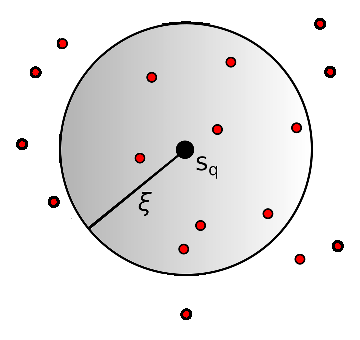
\includegraphics[width=.3\textwidth]{dados/figuras/rqu.eps}
\caption{Exemplo de consulta por abrangência}
\fonte{Autoria Própria}
\label{fig:exemplorq}
\end{figure}

A figura \ref{fig:exemplorq} exemplifica este tipo de consulta. Tomando $s_q$ e $\xi$ como parâmetros da consulta, todos os
elementos contidos pelo raio de abrangência fazem parte do conjunto resposta da consulta. $s_q$ não necessariamente precisa
pertencer ao conjunto de dados de pesquisa, devendo apenas pertencer ao mesmo domínio de dados.


Uma consulta aos k-vizinhos mais próximos \textit{kNNq($s_q$, $k$)} também recebe como um de seus parâmetros um elemento central da consulta $s_q$, e um número inteiro $k$ de vizinhos desejados, e retorna
como resultado o conjunto dos $k$ elementos com a menor dissimilaridade em relação ao elemento central da consulta $s_q$ \cite{POLA2010}.

\begin{mydef}
  \label{def:def_knnq}
  Seja $S$ um atributo complexo de um domínio $\mathbb{S}$ sobre o qual a condição de similaridade é expressada, seja $d$ uma
  função de distância, seja $k \in \mathbb{N^*}$ a quantidade de elementos desejados e seja $s_q \in \mathbb{S}$ o elemento
  central de consulta. A consulta kNNq($s_q$ , $k$) retorna $k$ elementos $s_i \in \mathbb{S}$ que possuem o valor do atributo $S$ menos distantes do valor 
  deste atributo referente ao elemento central da consulta\cite{Ferreira2009}:
  \begin{equation} \label{eq:knnq}   
    kNNq(s_q, k): S = \{s_i \in S \ |\  \forall \ s_j \in S - S^{'}, d(s_i, s_q)\leq d(s_j, s_q)\},
  \end{equation}
  onde $S^{'}$ = 0, se i = 1 e $S^{'}$ = \{$s_1$, ....., $s_{(i-1)}$\}, se 1 < i $\leq$ k. 
\end{mydef}

A figura \ref{fig:exemploknnq} exemplifica este tipo de operação. Nesta consulta, os parâmetros foram o elemento central da consulta $s_q$ e o número de elementos $k$ a serem
encontrados igual a 4. Os elementos ligados ao elemento central foram os mais próximos a este, portanto apenas eles fazem parte do conjunto resposta da consulta.
\begin{figure}[H]
\centering
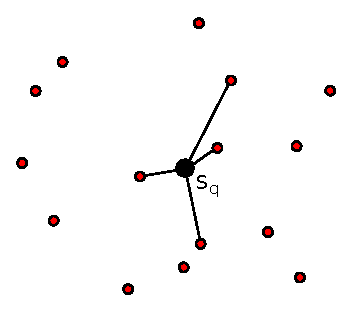
\includegraphics[width=.3\textwidth]{dados/figuras/knnq.eps}
\caption{Exemplo de consulta por k-vizinhos mais próximos}
\label{fig:exemploknnq}
\fonte{Autoria Própria}
\end{figure}

O SGBDR não possui suporte nativo a estes tipos de consulta, mas é possível construir estas consultas utilizando ferramentas existentes em um banco de dados relacional (como a \textit{B-tree}).\par %escopo do trabalho

A solução abordada por esta proposta é a do uso de técnicas Omni, presentes no trabalho de \cite{Traina2001}. Um número calculado de elementos do conjunto de dados são selecionados como "focos", e utilizados para
podar cálculos desnecessários de distâncias, fazendo uso da desigualdade triangular. 

A base da técnica Omni é calcular previamente as distâncias de todos os elementos para todos os focos selecionados, armazenando estas distâncias no banco. Quando uma consulta por similaridade
(como uma consulta por abrangência) é realizada, são conhecidas as distâncias entre o elemento central da consulta $s_q$ e o raio de abrangência $\xi$. Considerando um foco ${f_1}$ e utilizando
a desigualdade triangular, elementos que possuem uma distância entre o foco escolhido menor do que a distância de $s_q$ até o foco menos o valor $\xi$ serão descartados do conjunto de elementos necessários para
os cálculos de distância com o elemento central. Simetricamente, elementos cuja distância até o foco seja maior do que a distância de $s_q$ até o foco mais o valor do raio de abrangência $\xi$ também
serão descartados. Com isso, ocorre uma grande redução do número de cálculos necessários para fornecer o conjunto resposta. Essa poda também pode ser realizada por mais de um foco.

\begin{figure}[H]
\centering
\caption{Consulta por abrangência pela técnica Omni utilizando um foco}
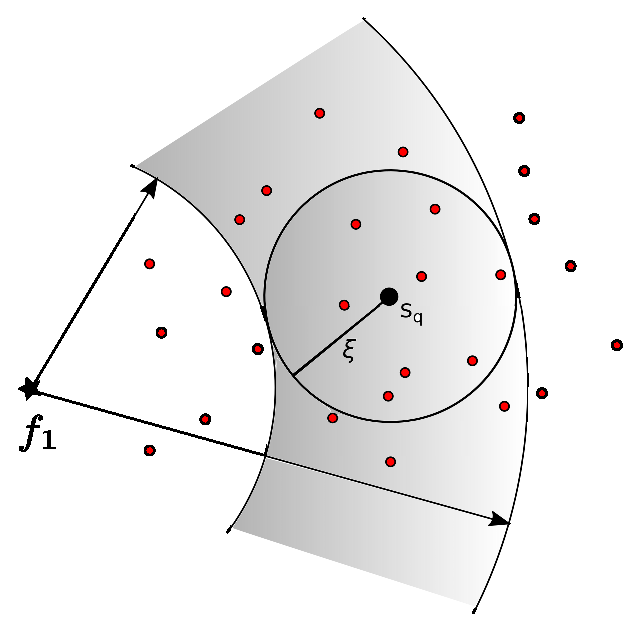
\includegraphics[width=.4\textwidth]{dados/figuras/rg_omni_1.eps}
\fonte{Autoria Própria}
\label{fig:rqomni1}
\end{figure}


A figura \ref{fig:rqomni1} ilustra a poda no número de cálculos. Apenas os elementos na área sombreada terão as suas distâncias em relação ao centro da consulta calculadas, pois estão no
conjunto de elementos que não foram descartados utilizando a desigualdade triangular com as distâncias previamente calculadas em relação ao foco. O armazenamento das distâncias de cada foco ${f_i}$ para cada outro elemento $s_k$ será feito 
utilizando uma estrutura de indexação que implementa os conceitos da técnica Omni com a estrutura da B-tree, originando uma nova estrutura chamada de OmniB-Tree. As distâncias serão armazenadas em $l$ OmniB-Trees, sendo $l$ o número de focos
criados para a base de dados \cite{Traina2001}.

\section{OBJETIVOS}
\label{sec:objetivos}
Os objetivos encontram-se divididos em objetivos gerais, referentes ao resultado obtido com a conclusão deste trabalho e objetivos específicos, ilustrando etapas intermediárias necessárias para alcançar o objetivo geral.
\subsection{OBJETIVOS GERAIS}
\label{subsec:objger}
O principal foco deste trabalho é a construção de um sistema de consultas por similaridade em uma base de imagens utilizando técnicas da família Omni para reduzir o custo computacional das operações de consulta.

\subsection{OBJETIVOS ESPECÍFICOS}
\label{subsec:objesp}
\begin{itemize}
 \item Modelar o banco de dados para atender a problemática apresentada;
 \item Aplicar os extratores de características das imagens utilizadas;
 \item Inserir no banco de dados as imagens e os valores de suas características;
 \item Criar a estrutura Omni necessária para a filtragem dos cálculos;
 \item Analisar e comparar os resultados obtidos.
\end{itemize}


\section{ORGANIZAÇÃO DO TRABALHO}
\label{sec:organizacaoTrabalho}

A estrutura deste trabalho apresenta mais detalhes sobre os tipos de consulta por similaridade utilizados, assim como os seus algoritmos computacionais. Posteriormente, explana os conceitos e técnicas da família Omni utilizada para
melhorar a performance das consultas. Também realiza a abordagem sobre os extratores de características utilizados para a base de imagens utilizada neste trabalho.
                		           % Introdução
% REVISÃO DE LITERATURA--------------------------------------------------------

\chapter{REVISÃO DE LITERATURA}
\label{chap:fundamentacaoTeorica}

É uma boa prática iniciar cada novo capítulo com um breve texto introdutório (tipicamente, dois ou três parágrafos) que deve deixar claro o quê será discutido no capítulo, bem como a organização do capítulo.
Também servirá ao propósito de "amarrar"{} o conteúdo deste capítulo com o conteúdo do capítulo imediatamente anterior.
         % Revisão de Literatura
% METODOLOGIA------------------------------------------------------------------

\chapter{METODOLOGIA}
\label{chap:metodologia}
Cada capítulo deve conter uma pequena introdução (tipicamente, um ou dois parágrafos) que deve deixar claro o objetivo e o que será discutido no capítulo, bem como a organização do capítulo.

\section{DELINEAMENTO DA PESQUISA}
\label{sec:titSecDelPesq}

Inserir seu texto aqui...

\section{COLETA E TRATAMENTO DE DADOS}
\label{sec:titSecColDad}

Inserir seu texto aqui...

                   % Metodologia
% RESULTADOS-------------------------------------------------------------------

\chapter{RESULTADOS}
\label{chap:resultados}

Este capítulo ilustra como foram feitas as etapas de implementação, detalhando alguns fatores importantes nos códigos utilizados, métodos para a descoberta ótima do número de focos para cada base,
assim como uma breve explicação sobre as bases de dados utilizadas e algunas das métricas empregadas. Também apresenta os resultados
obtidos, e análises pertinentes a estes resultados, estabelecendo um comparativo com as técnicas convencionais de pesquisa por similaridade. Todos os resultados foram extraídos utilizando o SGBD
PostgreSQL 10.3 em conjunto com o aplicativo pgAdmin 4 versão 2.1, responsável pela interface com o banco de dados. O hardware utilizado para as pesquisas é um Intel® Core i7™ 7700HQ 2.8 GHz possuindo 16 GB de memória RAM.
O sistema operacional utilizado foi o Windows 10 Home Edition.


\section{BASES DE DADOS}
\label{sec:basesdedados}
Foram utilizadas duas bases de dados complexas distintas para a verificação deste trabalho: uma base de imagens de cães e gatos, e uma
base de dados extraídos de exames médicos de imagem.

\catcode`\_=13 
\def_{\textunderscore}
\subsection{BASE CAT_DOG}
\catcode`_=8
\label{subsec:catdog}
Esta base de dados é dividida entre conjunto de teste e conjunto de treinamento, e encontra-se disponível em \href{https://www.kaggle.com/c/dogs-vs-cats}{<https://www.kaggle.com/c/dogs-vs-cats>}.
A base originalmente foi criada para uma competição promovida pela comunidade de cientistas de dados conhecida como Kaggle, aonde o objetivo era criar o algoritmo que conseguisse classificar imagens
entre fotografias ou desenhos de gatos ou cachorros com o maior índice de acerto. 

Para a verificação da técnica implementada, foi utilizado o conjunto de imagens de treino, com 25000 imagens, divididas igualmente entre cães e gatos. 
Tornou-se necessário a remoção de 3 imagens que eram pequenas demais e impossibilitavam a segmentação destas na etapa de processamento de imagens. As imagens foram processadas para a extração
das características desejadas e inseridas no banco de dados. As características escolhidas para cor foram a média e a variância do valor dos pixels em cada um dos três canais, para textura
foram dissimilaridade, contraste e correlação, e para a característica de forma foram utilizadas métricas como área, excentricidade e a razão área sobre área convexa. Todas as características
foram extraídas utilizando um script feito na linguagem Python versão 3.5, com o auxílio da biblioteca de algoritmos de manipulação de imagens \textit{scikit-image}.
\begin{figure}[H]
  \centering
  \subfloat[cat.325]{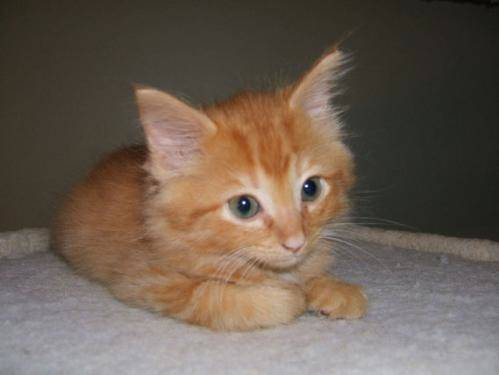
\includegraphics[width=.20\textwidth]{dados/figuras/cat325.jpg}} \hspace{2cm}
  \subfloat[cat.6243]{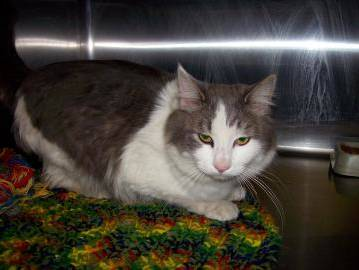
\includegraphics[width=.20\textwidth]{dados/figuras/cat6243.jpg}} \\
  \subfloat[dog.2032]{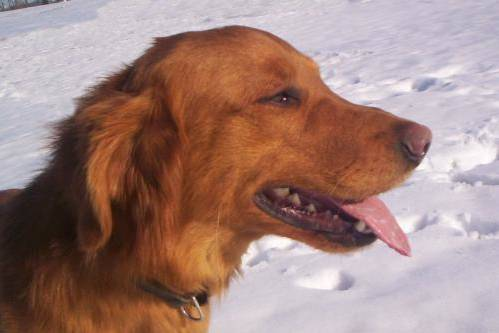
\includegraphics[width=.20\textwidth]{dados/figuras/dog2032.jpg}}\hspace{2cm}
  \subfloat[dog.10641]{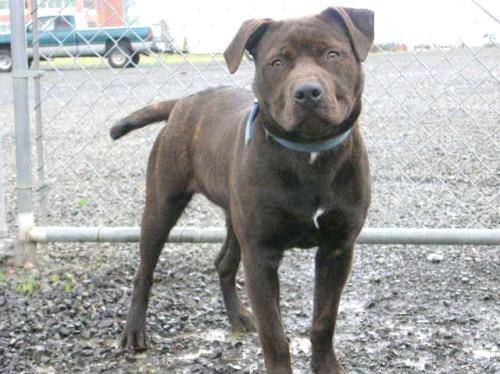
\includegraphics[width=.20\textwidth]{dados/figuras/dog10641.jpg}} 
  \caption{Exemplos de imagens da base CAT\_DOG}
\label{fig:catdogex}
\end{figure}

\subsection{BASE HC}

A base HC foi fornecida pelo Hospital das Clínicas de Ribeirão Preto, e ela consiste em 500000 imagens com as suas características já extraídas de uma base de imagens no formato DICOM. Embora ela seja uma base não-sintética, não foram fornecidos as imagens correspondentes aos vetores de características,
tornando-se assim impossível realizar uma análise qualitativa sobre a taxa de acerto nas buscas por similaridade mas ainda é possível verificar o tempo de consulta nesta base, fator este que é o interesse deste trabalho.

Os dados se encontram na forma de vetores, com a primeira posição sendo um número inteiro utilizado como um identificador da coluna seguido por um vetor de 256 números decimais, representando as características extraídas de 256 tons de cinza de cada imagem. Embora esta base não
possua as imagens correspondentes aos dados extraídos, o seu tamanho e a sua complexidade são maiores do que a base apresentada em \ref{subsec:catdog}, tornando mais evidente os ganhos de performance nas consultas por similaridade utilizando a técnica proposta.


\section{MÉTRICAS DOS TESTES}
\label{sec:metricas}
As métricas utilizadas nos testes foram os tempos gastos pelo pgAdmin para planejar e executar as consultas. Estas métricas foram adquiridas através dos comandos \textit{EXPLAIN ANALYZE} seguido da consulta a ser realizada, como por exemplo abaixo.
\begin{lstlisting}[caption={Exemplo de comando utilizado para a visualização das métricas de performance}, captionpos=t,basicstyle=\tiny]
EXPLAIN ANALYZE SELECT * FROM rangeOmniHCF2(12345, 30)
\end{lstlisting}

Os testes foram feitos escolhendo um centro de pesquisa aleatoriamente, e variando os parâmetros de raio para o caso da consulta por abrangência, e
os valores de $k$ para uma consulta do tipo $k$-vizinhos mais próximos. Também foi utilizado o número de podas de cálculos desnecessários de distância, conseguidos pela técnica aplicada neste trabalho.

\subsection{EXPLAIN ANALYZE}
O comando \textit{EXPLAIN ANALYZE} utilizado para a verificação dos tempos gastos pelo SGBD para a realização das consultas é nativo exclusivamente do PostgreSQL. O comando é utilizado para
mostrar o plano de execução gerado para uma declaração, sem executá-la. As tabelas referenciadas, assim como algoritmos de junção ou índices utilizados são
explicitados pelo \textit{EXPLAIN} \cite{POSTGRESQL2017}. Em associação com o comando \textit{ANALYZE}, a declaração também é executada e as estatísticas relacionadas ao tempo de execução atuais são mostradas para o usuário, divididas entre templo de planejamento e tempo de execução.

\subsubsection{TEMPO DE PLANEJAMENTO}
O tempo de planejamento (\textit{planning time}) é o tempo gasto pelo SGBD para planejar a maneira mais rápida de executar a consulta. O plano escolhido
é aquele que possui a execução estimada menos custosa dentre diversos outros planos testados pelo planejador. No contexto deste trabalho, o tempo de planejamento 
é pequeno o bastante para ser desprezado, representando um pouco mais de 1\% do tempo gasto no caso da consulta mais rápida, e menos de 0,001\% no caso mais lento. Os tempos de planejamento ficaram em uma média de 0.023 ms para
pesquisas na base cat\_dog e 0.027 ms para pesquisas na base HC.

\subsubsection{TEMPO DE EXECUÇÃO}
O tempo de execução (\textit{execution time}) representa o tempo em que o sistema leva para para executar o plano de consulta escolhido, além do tempo gasto para retornar 
a resposta da consulta para o usuário. Para o mérito de análise do ganho de performance utilizando a técnica OMNI, esta será a métrica utilizada. Este tempo é influenciado pela
complexidade da consulta, tamanho da base de dados, presença ou não de índices e hardware utilizado para a sua execução. 

\section{NÚMERO DE FOCOS}
Como mencionado no Capítulo \ref{chap:omni}, a escolha do número de focos impacta diretamente na performance da técnica OMNI. Se o número for menor que o ótimo, a \textit{mbOr} torna-se
muito grande, e o número de podas de cálculos diminui, aumentando assim o tempo de execução. Se o número de focos for maior que o ótimo, existe pouca variação na \textit{mbOr} mas o número de cálculos necessários para
descobrir a pertinência na região aumenta, aumentando o tempo de execução. O cálculo da dimensão intrínseca da base de dados pela técnica de box-counting não é realizável para bases
clusterizadas \cite{Mo2012} e normalizar as coordenadas de uma base de dados deste tipo seria alterar as informações originais salvas nas tabelas, alterando assim o dado armazenado. Uma solução
proposta por este trabalho provém da contagem do número de podas.

O número ótimo de focos é obtido analisando um gráfico do número de podas em relação ao número de focos utilizados. Um número ótimo de focos é aquele que produz um número suficiente de podas sem afetar o desempenho para a aplicação delas.
Como ilustrado pelas Figuras \ref{fig:focoHC} e \ref{fig:fococatdog}, os números ótimos de focos para as bases HC e cat\_dog são respectivamente 2 e 1.

% O número de focos tem influência no desempenho das consultas. Mas, existe uma relação custo/benefício para o número de focos 
% utilizados, pois quanto mais focos utilizados, maior o custo da aplicação de podas. Um número ótimo de focos é aquele que % produz um número suficiente de podas sem afetar o desempenho para a aplicação delas. Isso pode ser averiguado 
% analisando-se um gráfico


\begin{figure}[H]
\centering
\caption{Número de podas por focos utilizados para a base HC}
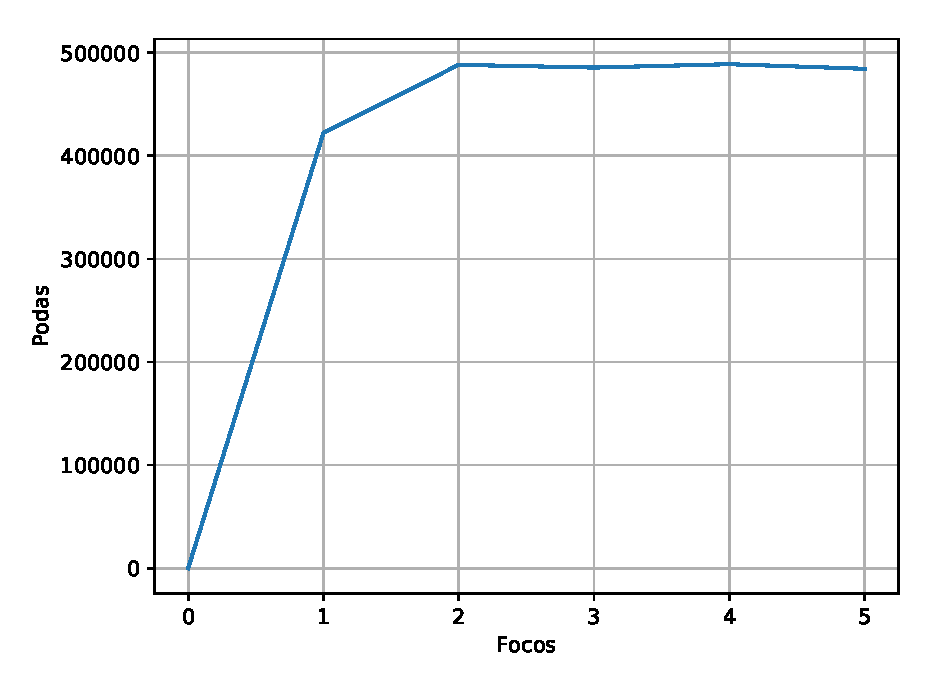
\includegraphics[width=.6\textwidth]{dados/figuras/focoHC.eps}
\fonte{Autoria Própria}
\label{fig:focoHC}
\end{figure}

\begin{figure}[H]
\centering
\caption{Número de podas por focos utilizados para a base cat\_dog}
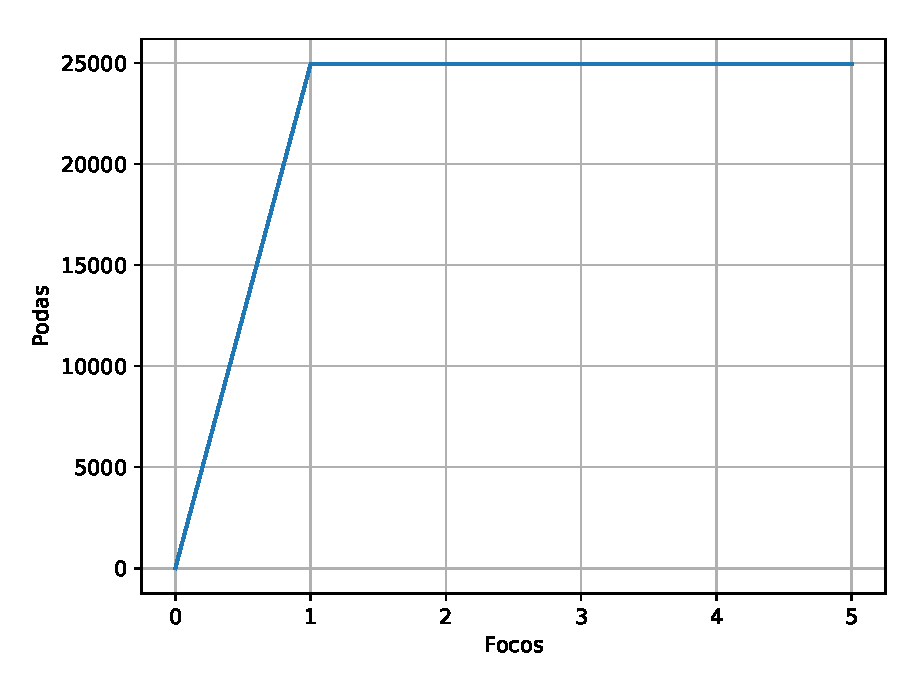
\includegraphics[width=.6\textwidth]{dados/figuras/fococatdog.eps}
\fonte{Autoria Própria}
\label{fig:fococatdog}
\end{figure}

\section{SCRIPTS SQL}
Os scripts necessários para a parte de manipulação do banco de dados foram todos escritos em PLPGSQL, uma linguagem estrutural estendida da SQL, desenvolvida para o uso
no SGBD PostgreSQL. Também foi utilizada a extensão \textit{cube} presente no PostgreSQL, para o cálculo das distâncias. Aqui serão discutidos apenas alguns scripts mais importantes para a análise de resultados. Os demais códigos encontram-se integralmente
nos Apêndices \ref{chap:apendice}. Para fins de otimização dos scripts (tanto sequenciais ou OMNI), tornou-se necessário
a criação de uma função para cada par (atributo, distância) envolvendo a base de dados cat\_dog.

\subsection{SCRIPTS SEQUENCIAIS}
Os scripts sequenciais das consultas realizam a pesquisa vasculhando toda a base de dados, e retornando os elementos que fazem
parte do critério de seleção, seja dentro do raio de abrangência indicado, ou dentre os $k$ elementos mais próximos do elemento central.
Abaixo, códigos utilizados para consultas sequenciais na base cat\_dog.

\begin{lstlisting}[caption={Consulta por abrangência sequêncial utilizando forma e distância euclidiana\\}, captionpos=t,basicstyle=\tiny] 
CREATE OR REPLACE FUNCTION rangeQueryShapeL2 (center_id integer, radius FLOAT8) 
RETURNS SETOF genericQuery AS $$
BEGIN
	  RETURN QUERY SELECT DISTINCT * FROM 
	  (SELECT T2.id_ft, (cube(T1.feature) <-> cube(T2.feature)) AS dist -- <-> indica calculo de
	  FROM SHAPE T1, SHAPE T2 WHERE T1.id_ft = center_id) 		    -- distancia L2
	  AS quer WHERE dist <= radius ORDER BY dist;	
END;$$
LANGUAGE PLPGSQL;
\end{lstlisting}

\begin{lstlisting}[caption={Consulta k-vizinhos mais próximos sequêncial utilizando cor e distância city-block}, captionpos=t,basicstyle=\tiny]
CREATE OR REPLACE FUNCTION kNNColorL1 (center_id integer, k_neigh integer) 
RETURNS SETOF genericQuery AS $$
BEGIN
	RETURN QUERY SELECT * FROM 
	(SELECT T2.ID_FT, (cube(T1.feature) <#> cube(T2.feature)) AS dist  -- <#> indica calculo de 
	FROM COLOR T1, COLOR T2 WHERE T1.id_ft = center_id 		   -- distancia L1
	AND T1.ID_FT <> T2.ID_FT) as quer 
	ORDER BY dist LIMIT k_neigh;	
END;$$
LANGUAGE PLPGSQL;
\end{lstlisting}

Como a base HC apresenta apenas um grande vetor como característica, foram necessárias apenas 3 funções, uma para cada distância Minkowski utilizada.

\begin{lstlisting}[caption={Consulta por abrangência sequêncial utilizando distância Chebyshev para a base HC}, captionpos=t, basicstyle=\tiny]
CREATE OR REPLACE FUNCTION rq_HC_LInf (center_id integer, radius FLOAT8) 
RETURNS SETOF genericQuery AS $$
BEGIN
	RETURN QUERY SELECT DISTINCT * FROM 
	(SELECT T2.COD, (cube(T1.feature) <=> cube(T2.feature)) AS dist   -- <-> indica calculo de
	FROM HC_TABLE T1, HC_TABLE T2 WHERE T1.cod = center_id) as quer   -- distancia LInfinite
	WHERE dist <= radius ORDER BY dist;		
END;$$
LANGUAGE PLPGSQL;
\end{lstlisting}

\subsection{SCRIPTS OMNI}
Para um melhor uso do ganho de desempenho proposto pela técnica OMNI, observou-se a necessidade de criação de uma função para cada tripla (atributo, distância, número de focos). Isto se deve ao fato de que funções em SQL que possuem
o nível de flexibilidade necessário para a passagem de parâmetros como atributo, distância e número de focos utilizados, apresentam uma performance muito inferior quando comparadas com as suas versões \textit{hard-coded}. Além disso, a técnica OMNI
exige uma preparação inicial do banco e a criação das suas estruturas, como mencionado na Seção \ref{sec:tiposconsultas}. Os scripts necessários para essa preparação encontram-se no Apêndice \ref{chap:apendice}. Abaixo, códigos utilizados para 
as consultas OMNI.

\begin{lstlisting}[caption={rangeOmni utilizando 1 foco para a base cat\_dog}, captionpos=t, basicstyle=\tiny, label=code:omni1]
CREATE OR REPLACE FUNCTION rangeOmniShapeL2F1 (center_id integer, radius FLOAT8) 
RETURNS SETOF genericQuery AS $$
DECLARE rec_id RECORD; feature_aux FLOAT8[]; distance FLOAT8; dist_fc FLOAT8;
BEGIN
	SELECT T1.feature INTO feature_aux FROM Shape T1 WHERE T1.id_ft = center_id;
	SELECT dist_l2 INTO dist_fc FROM SHAPE_F_BASE where id_feature = center_id;	
	FOR rec_id IN SELECT id_feature FROM SHAPE_F_BASE 
	WHERE ((dist_l2 < (radius + dist_fc)) AND (dist_l2 > dist_fc - radius)) LOOP
	  SELECT (cube(feature_aux) <-> cube(feature)) 
	  INTO distance FROM SHAPE T1 
	  WHERE rec_id.id_feature = T1.id_ft ;
	  IF (distance < radius) THEN
	    RETURN NEXT (rec_id.id_feature, distance);			       
	  END IF;				
	END LOOP;
END;$$
LANGUAGE PLPGSQL;
\end{lstlisting}

Alguns elementos importantes do Código \ref{code:omni1} requerem uma explanação. Na linhas 3 nota-se a criação de variáveis para o armazenamento de alguns dados lidos. Isto é necessário para armazenar informações importantes
para a consulta em memória, evitando assim o acesso desnecessário a disco que é mais custoso que o acesso à memória. A linha 8 é a responsável pela checagem da pertinência à \textit{mbOr}, 
dada pela desigualdade triangular indicada pela Equação \ref{eq:omnirq}. Da linha 9 até a linha 13 nota-se a etapa de refinamento da técnica, necessária para eliminar elementos que não fazem parte do conjunto-resposta.

Códigos que utilizam mais de um foco apresentam a mesma estrutura, sendo a única diferença a interseção das múltiplas regiões, necessitando $l$ comparações de desigualdade triangular, sendo $l$ o número de focos da base. Essa diferença
é ilustrada na linha 10 do Código \ref{code:omni2}.
\begin{minipage}{\textwidth}
\begin{lstlisting}[caption={rangeOmni utilizando 2 focos para a base HC}, captionpos=t, basicstyle=\tiny, label=code:omni2]
CREATE OR REPLACE FUNCTION rangeOmniHCL2F2 (center_id integer, radius FLOAT8) 
RETURNS SETOF genericQuery AS $$
DECLARE rec_id RECORD; feature_aux FLOAT8[]; distance FLOAT8; dist_fc FLOAT8[];
BEGIN
      SELECT T1.feature INTO feature_aux FROM HC_TABLE T1 WHERE T1.cod = center_id;
      dist_fc = ARRAY(SELECT DISTINCT dist_l2 FROM HC_F_BASE WHERE id_feature = center_id); 
      FOR rec_id IN SELECT id_feature FROM HC_F_BASE 
      WHERE ((dist_l2 < (radius + dist_fc[1])) 
      AND (dist_l2 > dist_fc[1] - radius)) 
      INTERSECT (SELECT id_feature FROM HC_F_BASE 
      WHERE ((dist_l2 < (radius + dist_fc[2])) 
      AND (dist_l2 > dist_fc[2] - radius))) LOOP
	      SELECT (cube(feature_aux) <-> cube(feature)) INTO distance 
	      FROM HC_TABLE T1 WHERE rec_id.id_feature = T1.cod ;
	      IF (distance < radius) THEN
		      RETURN NEXT (rec_id.id_feature, distance);			       
	      END IF;				
      END LOOP; 
END;$$
LANGUAGE PLPGSQL;
\end{lstlisting}
\vspace{0.2cm}
\end{minipage}

\section{TEMPOS DE CONSULTAS}
\label{sec:temp_cons}
Os tempos de consultas foram extraídos como explicados na Seção \ref{sec:metricas}. Os resultados foram obtidos através de uma média de 10 medições distintas, os valores dos centros de pesquisa foram escolhidos aleatoriamente antes
do início dos testes, e o mesmo valor de centro foi utilizado para melhor comparação dos resultados. É importante ressaltar que diferentes características como textura, cor e forma não apresentam alterações significativas
nos tempos de consulta. A Tabela \ref{tab:cd_range_l1} mostra os resultados obtidos para a base CAT\_DOG, com $S_q$ = 42412, $\xi$ = 100 e utilizando a característica de forma.

\begin{table}[!htb]
    \centering
    \caption[Busca por abrangência - CAT\_DOG - L1 - FORMA]{Busca por abrangência - CAT\_DOG - L1 - FORMA.
    \label{tab:cd_range_l1}}
   % \begin{tabular}{l l l l}
   \begin{tabular}{l c c c}
        \midrule
            &Tempo de Execução(ms)&Nº Podas de Cálculos\\
        \midrule
            Sequencial & 8,721 & - \\
            OMNI 1 Foco & 1,747 & 24935 \\
            OMNI 2 Focos & 5,201 & 24935 \\
            OMNI 3 Focos & 7,606 & 24935 \\
            OMNI 4 Focos & 10,107 & 24935 \\
            OMNI 5 Focos & 12,271 & 24935 \\
        \bottomrule
    \end{tabular}
\end{table}

É possível notar que a melhor performance foi obtida com o número ótimo de focos ilustrado pela Figura \ref{fig:fococatdog}. E isto também
pode ser observado nas Tabelas \ref{tab:cd_range_l2} e \ref{tab:cd_range_linf}, que contém os resultados do mesmo experimento anterior, mas para as distâncias
$L_2$ e $L_{\infty}$.

\begin{table}[H]
    \centering
    \caption[Busca por abrangência - CAT\_DOG - L2 - FORMA]{Busca por abrangência - CAT\_DOG - L2 - FORMA.
    \label{tab:cd_range_l2}}
   % \begin{tabular}{l l l l}
   \begin{tabular}{l c c c}
        \toprule
            &Tempo de Execução(ms)&Nº Podas de Cálculos\\
        \midrule
            Sequencial & 8,728 & - \\
            OMNI 1 Foco & 1,825 & 24935 \\
            OMNI 2 Focos & 4,988 & 24935 \\
            OMNI 3 Focos & 7,525 & 24935 \\
            OMNI 4 Focos & 8,994 & 24935 \\
            OMNI 5 Focos & 11,591 & 24935 \\
        \bottomrule
    \end{tabular}
\end{table}

\begin{table}[H]
    \centering
    \caption[Busca por abrangência - CAT\_DOG - L$_\protect\infty$ - FORMA]{Busca por abrangência - CAT\_DOG - L$_\protect\infty$ - FORMA.
    \label{tab:cd_range_linf}}
   % \begin{tabular}{l l l l}
   \begin{tabular}{l c c c}
        \toprule
            &Tempo de Execução(ms)&Nº Podas de Cálculos\\
        \midrule
            Sequencial & 8,805 & - \\
            OMNI 1 Foco & 2,051 & 24935 \\
            OMNI 2 Focos & 4,638 & 24935 \\
            OMNI 3 Focos & 8,563 & 24935 \\
            OMNI 4 Focos & 9,651 & 24935 \\
            OMNI 5 Focos & 11,626 & 24935 \\
        \bottomrule
    \end{tabular}
\end{table}

Outro fator a ser notado é o número de podas permaneceu constante independente do tipo de distância utilizada. Isto se deve ao fato
do valor das distâncias não variarem muito com diferentes distâncias Minkowski para esta base de dados. As Tabelas \ref{tab:cd_range_text} e \ref{tab:cd_range_color}
exemplificam o fato de que diferentes características utilizadas não alteram significativamente a performance
das consultas, como dito no início da Seção \ref{sec:temp_cons}. Para essa consulta, foram utilizados $S_q$ = 42413 e 42414 (característica de
textura e cor referente a mesma imagem da característica de forma com identificador = 42412) e $\xi$ = 100.

\begin{table}[H]
    \centering
    \caption[Busca por abrangência - CAT\_DOG - L1 - TEXTURA]{Busca por abrangência - CAT\_DOG - L1 - TEXTURA.
    \label{tab:cd_range_text}}
   % \begin{tabular}{l l l l}
   \begin{tabular}{l c c c}
        \toprule
            &Tempo de Execução(ms)&Nº Podas de Cálculos\\
        \midrule
            Sequencial & 8,710 & - \\
            OMNI 1 Foco & 1,531 & 24950 \\
            OMNI 2 Focos & 4,512 & 24950 \\
            OMNI 3 Focos & 6,838 & 24950 \\
            OMNI 4 Focos & 9,447 & 24950 \\
            OMNI 5 Focos & 11,182 & 24950 \\
        \bottomrule
    \end{tabular}
\end{table}

\begin{table}[H]
    \centering
    \caption[Busca por abrangência - CAT\_DOG - L1 - COR]{Busca por abrangência - CAT\_DOG - L1 - COR.
    \label{tab:cd_range_color}}
   % \begin{tabular}{l l l l}
   \begin{tabular}{l c c c}
        \toprule
            &Tempo de Execução(ms)&Nº Podas de Cálculos\\
        \midrule
            Sequencial & 8,334 & - \\
            OMNI 1 Foco & 1,675 & 24923 \\
            OMNI 2 Focos & 4,819 & 24923 \\
            OMNI 3 Focos & 8,073 & 24923 \\
            OMNI 4 Focos & 9,628 & 24923 \\
            OMNI 5 Focos & 12,925 & 24923 \\
        \bottomrule
    \end{tabular}
\end{table}

Para a base HC, também é possível verificar o ganho de performance obtido pela técnica OMNI. Como a base é significativamente maior e os dados mais complexos, o ganho
de performance é mais notável, como ilustram as Tabelas \ref{tab:hc_range} e \ref{tab:hc_range2}. Estas tabelas foram construídas utilizando consultas com $S_q$ = 49628 e $\xi$ = 20.
Novamente, a melhor performance pode ser observada com o número ótimo de focos indicado pela Figura \ref{fig:focoHC}.

\begin{table}[H]
    \centering
    \caption[Busca por abrangência - HC- L1]{Busca por abrangência - HC - L1.
    \label{tab:hc_range}}
   % \begin{tabular}{l l l l}
   \begin{tabular}{l c c c}
        \toprule
            &Tempo de Execução(ms)&Nº Podas de Cálculos\\
        \midrule
            Sequencial & 4566,851 & - \\
            OMNI 1 Foco & 448,105 & 484381 \\
            OMNI 2 Focos & 292,709 & 490599 \\
            OMNI 3 Focos & 361,712& 499406 \\
            OMNI 4 Focos & 462,795 & 499845 \\
            OMNI 5 Focos & 882,159 & 499937 \\
        \bottomrule
    \end{tabular}
\end{table}

\begin{table}[H]
    \centering
    \caption[Busca por abrangência - HC- L2]{Busca por abrangência - HC - L2.
    \label{tab:hc_range2}}
   % \begin{tabular}{l l l l}
   \begin{tabular}{l c c c}
        \toprule
            &Tempo de Execução(ms)&Nº Podas de Cálculos\\
        \midrule
            Sequencial & 4310,409 & - \\
            OMNI 1 Foco & 1215,435 & 422246 \\
            OMNI 2 Focos & 307,757 & 484381 \\
            OMNI 3 Focos & 556,683 & 485574 \\
            OMNI 4 Focos & 598,664 & 488229 \\
            OMNI 5 Focos & 952,008 & 488841 \\
        \bottomrule
    \end{tabular}
\end{table}

A técnica OMNI aplicada com a consulta por $k$-vizinhos mais próximos não conseguiu trazer resultados mais rápidos do que a
consulta sequencial. Isto se deve ao fato de que esta consulta efetua uma busca por abrangência em torno do elemento central de pesquisa, e 
retorna os $k$ valores mais próximos. Para isto, o valor do raio utilizado deve ser grande o bastante para retornar um número razoável
de elementos. O Código \ref{code:knnomni} ilustra como foram feitas as consultas OMNI-\textit{kNN}.
\begin{minipage}{\textwidth}
\begin{lstlisting}[caption={kNN-OMNI utilizando 2 focos para a base HC}, captionpos=t, basicstyle=\tiny, label=code:knnomni]
CREATE OR REPLACE FUNCTION kNNOmniHCL2F2 (center_id INTEGER, k_value INTEGER) 
RETURNS SETOF genericQuery AS $$
DECLARE radius FLOAT8 := 100;
BEGIN
	RETURN QUERY SELECT * 
	FROM rangeOMNIHCL2F2(center_id,radius) 
	ORDER BY distance LIMIT k_value;		
END;$$
LANGUAGE PLPGSQL; 
\end{lstlisting}
\vspace{2cm}
\end{minipage}

Outra forma implementada foi a expansão do raio em tempo de execução da consulta, caso seja pequeno demais para retornar
os $k$ elementos necessários, mas este método provou ser ainda menos eficiente que o previamente mencionado. A Tabela \ref{tab:knnHC}
contém os valores dos tempos de execução de uma consulta OMNI-\textit{kNN} com $s_q$ = 75003, $k$ = 30. O valor de $\xi$ utilizado para
efetuar a consulta foi de 100.


\begin{table}[H]
    \centering
    \caption[Busca OMNI-\textit{kNN} - HC- L2]{Busca OMNI-\textit{kNN} - HC - L2.
    \label{tab:knnHC}}
   % \begin{tabular}{l l l l}
   \begin{tabular}{l c c }
        \toprule
            &Tempo de Execução(ms)\\
        \midrule
            Sequencial & 4733,579  \\
            OMNI 1 Foco & 6519,995  \\
            OMNI 2 Focos & 6341,987  \\
            OMNI 3 Focos & 7490,256 \\
            OMNI 4 Focos & 7548,550 \\
            OMNI 5 Focos & 10348,541 \\
        \bottomrule
    \end{tabular}
\end{table}

O uso da distância $L_\infty$ na base de dados HC provou ser inviável. A distância Minkowski com $p = \infty$ essencialmente mede a 
maior diferença de valores entre duas dimensões quaisquer de dois pontos. Como a base possui os valores dos seus atributos entre 0 e 256, 
esta distância geralmente convergia para 256, tornando boa parte da base igualmente espaçada entre si, e entre os focos. Isto dificulta
a poda de elementos, tornando a técnica ineficaz nesta situação.

\section{ANÁLISE QUALITATIVA DAS CONSULTAS}

As consultas tanto sequenciais como OMNI retornam o mesmo resultado, sendo a diferença apenas a velocidade de execução da consulta. O foco deste trabalho
mantém-se apenas nos tempos das consultas, mas para ilustrar como seriam o retorno dessas consultas, seguem abaixo alguns exemplos
de consultas nas três características da base CAT\_DOG.

\begin{figure}[H]
  \centering
  \subfloat[cat.50 - $S_q$]{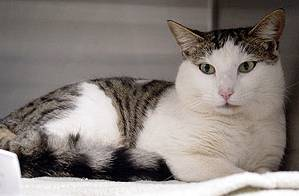
\includegraphics[width=.20\textwidth]{dados/figuras/cat50.jpg}} \hspace{2cm}
  \subfloat[cat.9211]{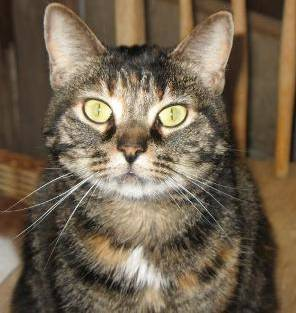
\includegraphics[width=.20\textwidth]{dados/figuras/cat9211.jpg}} \hspace{2cm}
  \subfloat[dog.10089]{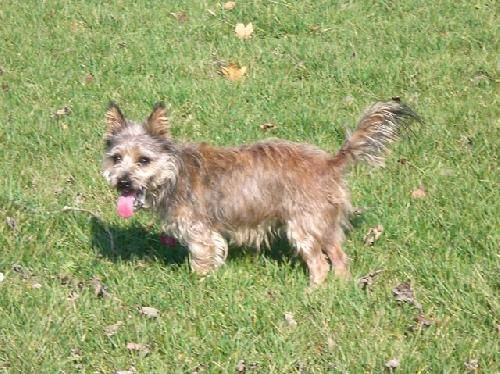
\includegraphics[width=.20\textwidth]{dados/figuras/dog10089.jpg}}\\
  \subfloat[dog.3125]{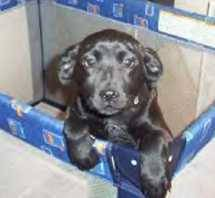
\includegraphics[width=.20\textwidth]{dados/figuras/dog3125.jpg}} \hspace{2cm}
  \subfloat[cat.5010]{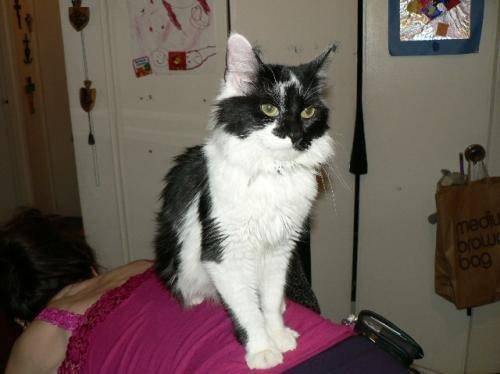
\includegraphics[width=.20\textwidth]{dados/figuras/cat5010.jpg}} \hspace{2cm}
  \subfloat[cat.4258]{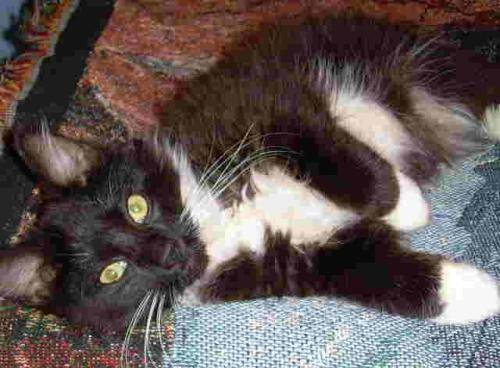
\includegraphics[width=.20\textwidth]{dados/figuras/cat4258.jpg}} \\
  \caption{Exemplo de consulta por abrangência utilizando Forma}
\end{figure}

\begin{figure}[H]
  \centering
  \subfloat[dog.6431 - $S_q$]{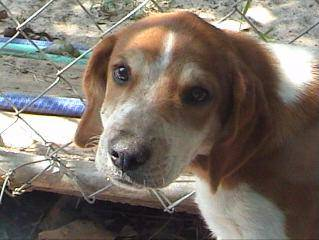
\includegraphics[width=.20\textwidth]{dados/figuras/dog6431.jpg}} \hspace{2cm}
  \subfloat[cat.3864]{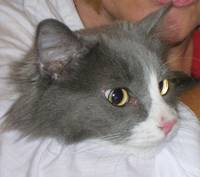
\includegraphics[width=.20\textwidth]{dados/figuras/cat3864.jpg}} \hspace{2cm}
  \subfloat[cat.6114]{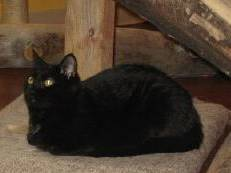
\includegraphics[width=.20\textwidth]{dados/figuras/cat6114.jpg}}\\
  \subfloat[cat.8027]{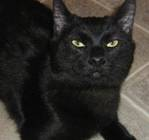
\includegraphics[width=.20\textwidth]{dados/figuras/cat8027}} \hspace{2cm}
  \subfloat[dog.12048]{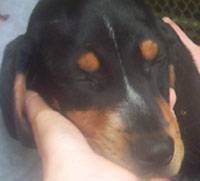
\includegraphics[width=.20\textwidth]{dados/figuras/dog12048.jpg}} \hspace{2cm}
  \subfloat[dog.4639]{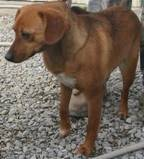
\includegraphics[width=.20\textwidth]{dados/figuras/dog4639.jpg}} \\
  \caption{Exemplo de consulta por abrangência utilizando Textura}
\end{figure}

\begin{figure}[H]
  \centering
  \subfloat[dog.11868 - $S_q$]{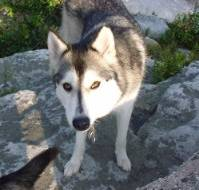
\includegraphics[width=.20\textwidth]{dados/figuras/dog11868.jpg}} \hspace{2cm}
  \subfloat[cat.12219]{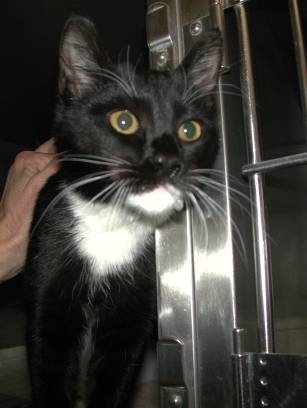
\includegraphics[width=.20\textwidth]{dados/figuras/cat12219.jpg}} \hspace{2cm}
  \subfloat[dog.9322]{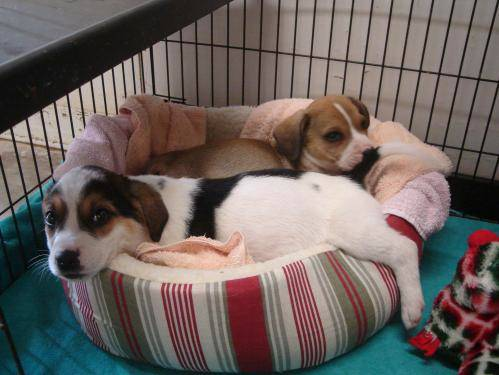
\includegraphics[width=.20\textwidth]{dados/figuras/dog9322.jpg}}\\
  \subfloat[cat.9185]{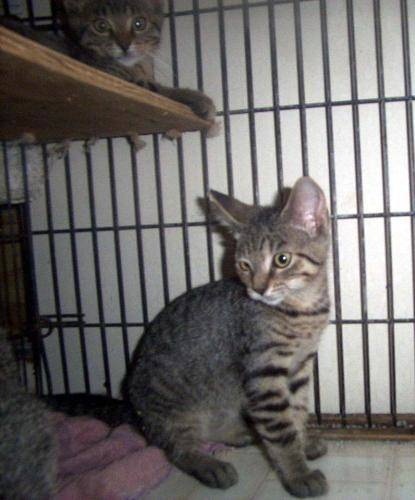
\includegraphics[width=.20\textwidth]{dados/figuras/cat9185}} \hspace{2cm}
  \subfloat[cat.4439]{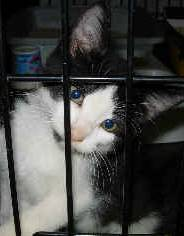
\includegraphics[width=.20\textwidth]{dados/figuras/cat4439.jpg}} \hspace{2cm}
  \subfloat[dog.10028]{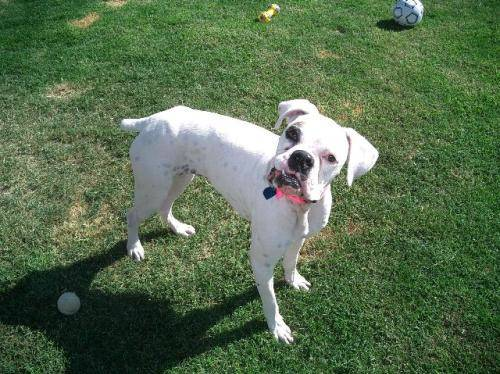
\includegraphics[width=.20\textwidth]{dados/figuras/dog10028.jpg}} \\
  \caption{Exemplo de consulta por abrangência utilizando Cor}
\end{figure}


\section{LIMITAÇÕES DA TÉCNICA}
\label{sec:limit}
Embora a técnica OMNI mostrou-se eficaz para consultas por abrangência mesmo em bases pequenas e com baixo nível de complexidade,
algumas limitações são inerentes à natureza da técnica. A principal limitação é em relação ao tamanho do raio $\xi$ empregado em consultas OMNI.
Quanto maior o raio, menos elementos são descartados pela etapa de poda, sendo necessário mais cálculos de pertinência à \textit{mbOr} e mais cálculos
de distância. As Tabelas \ref{tab:limit1} e \ref{tab:limit2} mostram um comparativo do tempo de execução de consultas por abrangência sequenciais e OMNI conforme aumenta-se
o raio de pesquisa para as bases CAT\_DOG e HC, juntamente com o número de elementos do conjunto resposta.

\begin{table}[H]
    \centering
    \caption[Performance em função do aumento do raio - CAT\_DOG]{Performance em função do aumento do raio - CAT\_DOG.
    \label{tab:limit1}}
   % \begin{tabular}{l l l l}
   \begin{tabular}{c c c c}
        \toprule
           Raio &Sequencial (ms)&OMNI (ms) &Nº Elementos\\
        \midrule
            100 & 8,598 & 1,938 & 62 \\
            500 & 8,580 & 4,582 & 324 \\
            1000 & 8,951 & 7,91 & 633 \\
            1500 & 8,760 & 11,119 & 973 \\
            2000 & 9,164 & 12,735 & 1331 \\
            2500 & 9,518 & 16,379 & 1654 \\
            3000 & 10,307 & 20,153 & 2000 \\
            3500 & 10,466 & 25,228 & 2303 \\
            4000 & 10,464 & 28,088 & 2597 \\
            4500 & 10,609 & 29,088 & 2928 \\
           
        \bottomrule
    \end{tabular}
\end{table}

\begin{table}[H]
    \centering
    \caption[Performance em função do aumento do raio - HC]{Performance em função do aumento do raio - HC.
    \label{tab:limit2}}
   % \begin{tabular}{l l l l}
   \begin{tabular}{c c c c}
        \toprule
           Raio &Sequencial (ms)&OMNI (ms) &Nº Elementos\\
        \midrule
            20 & 4742,696 & 254,221 & 11 \\
            50 & 4917,345 & 1122,165 & 553 \\
            80 & 4626,832 & 1890,589 & 2001 \\
            110 & 4762,850 & 2683,298 & 4256 \\
            140 & 4825,782 & 3531,885 & 7992 \\
            170 & 4708,758 & 8280,403 & 13903 \\
            200 & 4927,518 & 8251,041 & 22708 \\
            230 & 4893,118 & 8393,683 & 36753 \\
            260 & 5157,097 & 8800,501 & 59719 \\
            290 & 5415,949 & 9045,798 & 95710 \\
           
        \bottomrule
    \end{tabular}
\end{table}                    % Resultados
% ORIENTAÇÕES GERAIS------------------------------------------------------------


% SOBRE AS ILUSTRAÇÕES----------------------------------------------------------
\chapter{SOBRE AS ILUSTRAÇÕES}
\label{chap:apSobreIlust}

A seguir exemplifica-se como inserir ilustrações no corpo do trabalho. As ilustrações serão indexadas automaticamente em suas respectivas listas. A numeração sequencial de figuras, tabelas e equações também ocorre de modo automático.

Referências cruzadas são obtidas através dos comandos \verb|\label{}| e \verb|\ref{}|. Sendo assim, não é necessário por exemplo, saber que o número de certo capítulo é \ref{chap:fundamentacaoTeorica} para colocar o seu número no texto. Outra forma que pode ser utilizada é esta: \autoref{chap:fundamentacaoTeorica}, facilitando a inserção, remoção e manejo de elementos numerados no texto sem a necessidade de renumerar todos esses elementos.

% FIGURAS-----------------------------------------------------------------------
\chapter{FIGURAS}
\label{chap:figuras}

Exemplo de como inserir uma figura. A \autoref{fig:figura-exemplo1} aparece automaticamente na lista de figuras. Para saber mais sobre o uso de imagens no \LaTeX{} consulte literatura especializada \cite{Goossens2007}.

Os arquivos das figuras devem ser armazenados no diretório de "/dados".

\begin{figure}[!htb]
    \centering
    \caption{Exemplo de Figura}
    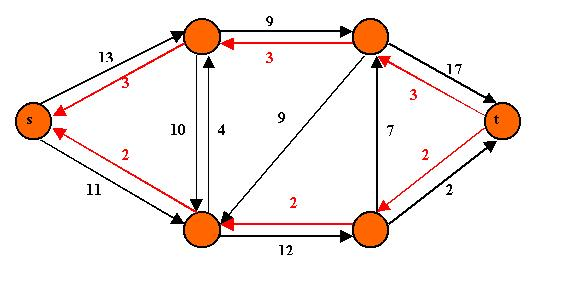
\includegraphics[width=0.5\textwidth]{./dados/figuras/figura1}
    \fonte{\citeonline{IRL2014}}
    \label{fig:figura-exemplo1}
\end{figure}

% QUADROS E TABELAS---------------------------------------------------------------
\chapter{QUADROS E TABELAS}
\label{chap:tabelas}

Exemplo de como inserir o \autoref{qua:quadro-exemplo1} e a \autoref{tab:tabela-exemplo1}. Ambos aparecem automaticamente nas suas respectivas listas. Para saber mais informações sobre a construção de tabelas no \LaTeX{} consulte literatura especializada \cite{Mittelbach2004}.

Ambos os elementos (Quadros e Tabelas) devem ser criados em arquivos separados para facilitar manutenção e armazenados no diretório de "/dados".

\begin{quadro}[!htb]
    %\centering
    \caption{Cronograma de Atividades.\label{qua:cronograma}}
    \begin{tabular}{|p{5.0cm}|p{0.6cm}|p{0.6cm}|p{0.6cm}|p{0.6cm}|p{0.6cm}|p{0.6cm}|p{0.6cm}|p{0.6cm}|p{0.6cm}|p{0.6cm}|}
        \hline
        \textbf{Atividades} 						     & 	   \textbf{Set}      & \textbf{Out} & \textbf{Nov} & \textbf{Dez} & \textbf{Jan} & \textbf{Fev} & \textbf{Mar} & \textbf{Abr} & \textbf{Mai} & \textbf{Jun} \\
        \hline
        \footnotesize{1. Estudo e acompanhamento da literatura}		     & X	             & X            &  		   & 		  &  		 &   	        &   	       &   	      & 	     & 		     \\
        \hline
        \footnotesize{2. Modelagem do problema} 				     & X	             & X            &  		   & 		  &  		 &   	        &   	       &   	      & 	     &                \\
        \hline
	\footnotesize{3. Verificação das estruturas Omni} 			     &  	             & X            & X		   & 		  &  		 &   	        &   	       &   	      & 	     &                \\
        \hline
	\footnotesize{4. Estudo dos extratores de características} 		     &  	             &              & X		   & 		  &  		 &   	        &   	       &   	      & 	     & 		     \\
        \hline
	\footnotesize{5. Estudo e inserção das métricas no banco} 		     &  	             & X            & X		   &  		  &  		 &   	        &   	       &   	      & 	     & 		     \\
        \hline
	\footnotesize{6. Criação e povoamento da base de dados} 		     &  	             &              & X		   & X		  &  		 &   	        &   	       &   	      & 	     & 		     \\
        \hline
        \footnotesize{7. Elaboração da apresentação do TCC1}			     &  	             &              & X		   & X		  &  		 &   	        &   	       &   	      & 	     & 		     \\
        \hline        
        \footnotesize{8. Defesa do TCC1}                                             &  	             &              &  		   & X		  &  		 &   	        &   	       &   	      & 	     & 		     \\
        \hline
	\footnotesize{9. Implementação da busca sequencial} 			     &  	             &              &  		   & 		  & X		 & X	        & X 	       &   	      & 	     & 		     \\
        \hline
        \footnotesize{10. Implementação da técnica Omni} 			     &  	             &              &  		   & 		  & X		 & X 	        & X 	       &   	      & 	     & 		     \\
        \hline
        \footnotesize{11. Comparação e análise de resultados} 			     &  	             &              &  		   & 		  &  		 &   	        &  X	       & X 	      & 	     & 		     \\
        \hline
        \footnotesize{12. Implementação da interface} 				     &  	             &              &  		   & 		  &  		 &   	        &  X	       &  X	      & 	     & 		     \\
        \hline
        \footnotesize{13. Elaboração da apresentação final} 			     &  	             &              &  		   & 		  &  		 &   	        &   	       &  X	      &  X	     & 		     \\
        \hline        
        \footnotesize{14. Defesa do TCC2}					     &  	             &              &  		   & 		  &  		 &   	        &   	       &   	      & 	     & X	     \\
        \hline
    \end{tabular}
\end{quadro}

%Estudo, modelagem, verificação das estruturas Omni, bases, extratores, métricas, criar o banco e inserir as métricas, implementação da Omni, implementação seq sem Omni, comparação

A diferença entre quadro e tabela está no fato que um quadro é formado por linhas horizontais e verticais. Deve ser utilizado quando o conteúdo é majoritariamente não-numérico. O número do quadro e o título vem acima do quadro, e a fonte, deve vir abaixo. E Uma tabela é formada apenas por linhas verticais. Deve ser utilizada quando o conteúdo é majoritariamente numérico. O número da tabela e o título vem acima da tabela, e a fonte, deve vir abaixo, tal como no quadro.

\begin{table}[!htb]
    \centering
    \caption[Resultado dos testes]{Resultado dos testes.
    \label{tab:tabela-exemplo1}}
    \begin{tabular}{rrrrr}
        \toprule
            & Valores 1 & Valores 2 & Valores 3 & Valores 4 \\
        \midrule
            Caso 1 & 0,86 & 0,77 & 0,81 & 163 \\
            Caso 2 & 0,19 & 0,74 & 0,25 & 180 \\
            Caso 3 & 1,00 & 1,00 & 1,00 & 170 \\
        \bottomrule
    \end{tabular}
    \fonte{\citeonline{Barbosa2004}}
\end{table}


% EQUAÇÕES-----------------------------------------------------------------------
\chapter{EQUAÇÕES}
\label{chap:equacoes}

Exemplo de como inserir a \autoref{eq:equacao-exemplo1} e a Eq. \ref{eq:equacao-exemplo2} no corpo do texto \footnote{Deve-se atentar ao fato de a formatação das equações ficar muito boa esteticamente.}. Observe que foram utilizadas duas formas distintas para referenciar as equações.

\begin{equation}
    X(s) = \int\limits_{t = -\infty}^{\infty} x(t) \, \text{e}^{-st} \, dt
    \label{eq:equacao-exemplo1}
\end{equation}

\begin{equation}
    F(u, v) = \sum_{m = 0}^{M - 1} \sum_{n = 0}^{N - 1} f(m, n) \exp \left[ -j 2 \pi \left( \frac{u m}{M} + \frac{v n}{N} \right) \right]
    \label{eq:equacao-exemplo2}
\end{equation}

% ALGORITMOS-----------------------------------------------------------------------
\chapter{ALGORITMOS}
\label{chap:algoritmos}

Exemplo de como inserir um algoritmo. Para inserção de algoritmos utiliza-se o pacote {\ttfamily algorithm2e} que já está devidamente configurado dentro do template.

Os algoritmos devem ser criados em arquivos separados para facilitar manutenção e armazenados no diretório de "/dados".\\
\\

\begin{algorithm}
    \caption{Exemplo de Algoritmo}
    \KwIn{o número $n$ de vértices a remover, grafo original $G(V, E)$}
    \KwOut{grafo reduzido $G'(V,E)$}
    $removidos \leftarrow 0$ \\
    \While {removidos $<$ n } {
        $v \leftarrow$ Random$(1, ..., k) \in V$ \\
            \For {$u \in adjacentes(v)$} {
                remove aresta (u, v)\\
                $removidos \leftarrow removidos + 1$\\
            }
            \If {há  componentes desconectados} {
                remove os componentes desconectados\\
            }
        }
\end{algorithm}


% SOBRE AS LISTAS--------------------------------------------------------------------
\chapter{SOBRE AS LISTAS}
\label{chap:apSobreLista}

Para construir listas de "\textit{bullets}"{} ou listas enumeradas, inclusive listas aninhadas, é utilizado o pacote \verb|paralist|.

Exemplo de duas listas não numeradas aninhadas, utilizando o comando \verb|\itemize|. Observe a indentação, bem como a mudança automática do tipo de "\textit{bullet}"{} nas listas aninhadas.

\begin{itemize}
    \item item não numerado 1
    \item item não numerado 2
    \begin{itemize}
        \item subitem não numerado 1
        \item subitem não numerado 2
        \item subitem não numerado 3
    \end{itemize}
    \item item não numerado 3
\end{itemize}

Exemplo de duas listas numeradas aninhadas, utilizando o comando \verb|\enumerate|. Observe a numeração progressiva e indentação das listas aninhadas.

\begin{enumerate}
    \item item numerado 1
    \item item numerado 2
    \begin{enumerate}
        \item subitem numerado 1
        \item subitem numerado 2
        \item subitem numerado 3
    \end{enumerate}
    \item item numerado 3
\end{enumerate}

% SOBRE AS CITAÇÕES E CHAMADAS DE REFERÊNCAS----------------------------------------------
\chapter{SOBRE AS CITAÇÕES E CHAMADAS DE REFERÊNCAS}
\label{chap:apSobreCita}

Citações são trechos de texto ou informações obtidas de materiais consultadss quando da elaboração do trabalho. São utilizadas no texto com o propósito de esclarecer, completar e embasar as ideias do autor. Todas as publicações consultadas e utilizadas (por meio de citações) devem ser listadas, obrigatoriamente, nas referências bibliográficas, para preservar os direitos autorais. São classificadas em citações indiretas e diretas.

% CITAÇÕES INDIRETAS-----------------------------------------------------------------------
\chapter{CITAÇÕES INDIRETAS}
\label{chap:citacoesLivres}

É a transcrição, com suas próprias palavras, das idéias de um autor, mantendo-se o sentido original. A citação indireta é a maneira que o pesquisador tem de ler, compreender e gerar conhecimento a partir do conhecimento de outros autores. Quanto à chamada da referência, ela pode ser feita de duas maneiras distintas, conforme o nome do(s) autor(es) façam parte do seu texto ou não. Exemplo de chamada fazendo parte do texto:\\
\\Enquanto \citeonline{Maturana2003} defendem uma epistemologia baseada na biologia. Para os autores, é necessário rever \ldots.\\

A chamada de referência foi feita com o comando \verb|\citeonline{chave}|, que produzirá a formatação correta.

A segunda forma de fazer uma chamada de referência deve ser utilizada quando se quer evitar uma interrupção na sequência do texto, o que poderia, eventualmente, prejudicar a leitura. Assim, a citação é feita e imediatamente após a obra referenciada deve ser colocada entre parênteses. Porém, neste caso específico, o nome do autor deve vir em caixa alta, seguido do ano da publicação. Exemplo de chamada não fazendo parte do texto:\\
\\Há defensores da epistemologia baseada na biologia que argumentam em favor da necessidade de \ldots \cite{Maturana2003}.\\

Nesse caso a chamada de referência deve ser feita com o comando \verb|\cite{chave}|, que produzirá a formatação correta.

% CITAÇÕES DIRETAS-----------------------------------------------------------------------
\chapter{CITAÇÕES DIRETAS}
\label{chap:citacoesLiterais}

É a transcrição ou cópia de um parágrafo, de uma frase, de parte dela ou de uma expressão, usando exatamente as mesmas palavras adotadas pelo autor do trabalho consultado.

Quanto à chamada da referência, ela pode ser feita de qualquer das duas maneiras já mencionadas nas citações indiretas, conforme o nome do(s) autor(es) façam parte do texto ou não. Há duas maneiras distintas de se fazer uma citação direta, conforme o trecho citado seja longo ou curto.

Quando o trecho citado é longo (4 ou mais linhas) deve-se usar um parágrafo específico para a citação, na forma de um texto recuado (4 cm da margem esquerda), com tamanho de letra menor e espaçamento entrelinhas simples. Exemplo de citação longa:
\\\begin{citacao}
    Desse modo, opera-se uma ruptura decisiva entre a reflexividade filosófica, isto é a possibilidade do sujeito de pensar e de refletir, e a objetividade científica. Encontramo-nos num ponto em que o conhecimento científico está sem consciência. Sem consciência moral, sem consciência reflexiva e também subjetiva. Cada vez mais o desenvolvimento extraordinário do conhecimento científico vai tornar menos praticável a própria possibilidade de reflexão do sujeito sobre a sua pesquisa \cite[p.~28]{Silva2000}.
\end{citacao}

Para fazer a citação longa deve-se utilizar os seguintes comandos:
\begin{verbatim}
\begin{citacao}
<texto da citacao>
\end{citacao}
\end{verbatim}

No exemplo acima, para a chamada da referência o comando \verb|\cite[p.~28]{Silva2000}| foi utilizado, visto que os nomes dos autores não são parte do trecho citado. É necessário também indicar o número da página da obra citada que contém o trecho citado.

Quando o trecho citado é curto (3 ou menos linhas) ele deve inserido diretamente no texto entre aspas. Exemplos de citação curta:\\
\\A epistemologia baseada na biologia parte do princípio de que "assumo que não posso fazer referência a entidades independentes de mim para construir meu explicar" \cite[p.~35]{Maturana2003}.\\
\\A epistemologia baseada na biologia de \citeonline[p.~35]{Maturana2003} parte do princípio de que "assumo que não posso fazer referência a entidades independentes de mim para construir meu explicar".

% DETALHES SOBRE AS CHAMADAS DE REFERÊNCIAS---------------------------------------------------------
\chapter{DETALHES SOBRE AS CHAMADAS DE REFERÊNCIAS}
\label{chap:referUtilizadas}

Outros exemplos de comandos para as chamadas de referências e o resultado produzido por estes:\\
\\\citeonline{Maturana2003} \ \ \  \verb|\citeonline{Maturana2003}|\\
\citeonline{Barbosa2004} \ \ \   \verb|\citeonline{Barbosa2004}|\\
\cite[p.~28]{Silva2000} \ \ \  \verb|\cite[p.~28]{Silva2000}|\\
\citeonline[p.~33]{Silva2000} \ \ \   \verb|\citeonline[p.~33]{v}|\\
\cite[p.~35]{Maturana2003} \ \ \   \verb|\cite[p.~35]{Maturana2003}|\\
\citeonline[p.~35]{Maturana2003} \ \ \   \verb|\citeonline[p.~35]{Maturana2003}|\\
\cite{Barbosa2004,Maturana2003} \ \ \   \verb|\cite{Barbosa2004,Maturana2003}|\\

% SOBRE AS REFERÊNCIAS BIBLIOGRÁFICAS-------------------------------------------------------
\chapter{SOBRE AS REFERÊNCIAS BIBLIOGRÁFICAS}
\label{chap:apSobreRefer}

A bibliografia é feita no padrão \textsc{Bib}\TeX{}. As referências são colocadas em um arquivo separado. Neste template as referências são armazenadas no arquivo "base-referencias.bib".

Existem diversas categorias documentos e materiais componentes da bibliografia. A classe abn\TeX{} define as seguintes categorias (entradas):

\begin{verbatim}
@book
@inbook
@article
@phdthesis
@mastersthesis
@monography
@techreport
@manual
@proceedings
@inproceedings
@journalpart
@booklet
@patent
@unpublished
@misc
\end{verbatim}

Cada categoria (entrada) é formatada pelo pacote \citeonline{abnTeX22014d} de uma forma específica. Algumas entradas foram introduzidas especificamente para atender à norma \citeonline{NBR6023:2002}, são elas: \verb|@monography|, \verb|@journalpart|,\verb|@patent|. As demais entradas são padrão \textsc{Bib}\TeX{}. Para maiores detalhes, refira-se a \citeonline{abnTeX22014d}, \citeonline{abnTeX22014b}, \citeonline{abnTeX22014c}.

% NOTAS DE RODAPÉ--------------------------------------------------------------------------
\chapter{NOTAS DE RODAPÉ}
\label{chap:notasRodape}

As notas de rodapé pode ser classificadas em duas categorias: notas explicativas\footnote{é o tipo mais comum de notas que destacam, explicam e/ou complementam o que foi dito no corpo do texto, como esta nota de rodapé, por exemplo.} e notas de referências. A notas de referências, como o próprio nome ja indica, são utilizadas para colocar referências e/ou chamadas de referências sob certas condições.

                   % Capítulo com Orientações de uso do Template
% CONCLUSÃO--------------------------------------------------------------------

\chapter{CONCLUSÃO}
\label{chap:conclusao}
No presente capítulo será abordada a conclusão do trabalho aqui escrito. Pontos fracos e pontos fortes da técnica utilizada, assim como cenários de melhor empregabilidade da técnica. Também serão discutidos possíveis aprimoramentos deste trabalho, na forma de
trabalhos ou pesquisas futuras.

\section{PERFORMANCE DA TÉCNICA}

Para as consultas por abrangência, a técnica OMNI conseguiu um ganho de performance significativo quando comparada com o método sequencial. A Tabela \ref{tab:performance1} mostra os ganhos de performance da consulta mais rápida em relação ao método
sequencial. O cálculo de ganho de performance (GP) percentual se dá por: $GP_\% = (T_o/T_s - 1)*100$, sendo $T_o$ o tempo da consulta OMNI mais rápida (quantidade de focos ótima) e $T_s$ o tempo da consulta sequencial.

\begin{table}[H]
    \centering
    \caption[Ganho de Performance - CAT\_DOG]{Ganho de Performance - CAT\_DOG.
    \label{tab:performance1}}
   % \begin{tabular}{l l l l}
   \begin{tabular}{l c}
        \toprule
            &GP (\%)\\
        \midrule
            L$_1$ - FORMA & 399,20 \\
            L$_2$ - FORMA & 378,24 \\
            L$_\infty$ - FORMA & 329,30 \\
            L$_1$ - TEXTURA & 468,91 \\
            L$_1$ - COR & 397,55 \\
        \bottomrule
    \end{tabular}
\end{table}

O ganho de performance para a base CAT\_DOG foi extremamente satisfatório, dado ao tamanho reduzido e baixa complexidade dos dados. Inicialmente estimou-se que a técnica só teria resultados significativos com bases massivas e com complexidade elevada, cenários
aonde a poda de cálculos desnecessários traria um maior benefício em questões de tempo de execução.

A base HC apresentou um ganho de performance ainda maior com a técnica OMNI, devido a sua elevada complexidade de dados e quantidade de tuplas a serem analisadas em cada consulta. Isto ilustra o potencial da técnica para bases ainda maiores, ou até mesmo para a manipulação
de \textit{Big Data}. A Tabela \ref{tab:performance2} contém os ganhos de performance da técnica na base HC.

\begin{table}[H]
    \centering
    \caption[Ganho de Performance - HC]{Ganho de Performance - HC.
    \label{tab:performance2}}
   % \begin{tabular}{l l l l}
   \begin{tabular}{l c}
        \toprule
            &GP (\%)\\
        \midrule
            L$_1$ & 1460,20 \\
            L$_2$ & 1304,04 \\
            L$_\infty$ & - \\
        \bottomrule
    \end{tabular}
\end{table}

Porém, a técnica tem as suas limitações, como visto na Seção \ref{sec:limit}. Enquanto consultas sequenciais apresentam pouca perda de desempenho com o aumento do raio da consulta por abrangência, as consultas OMNI são muito mais sensíveis às variações de raio.
Isso se deve ao fato de raios muito elevados causam um crescimento na \textit{mbOr}, o que acarreta em um número maior de alarmes falsos, aumentando a quantidade de cálculos de distância necessários na etapa de refinamento. Sob a luz dessas informações, é seguro dizer que 
a técnica OMNI só pode ser empregada viavelmente para consultas que retornem até no máximo cerca de 2\% do número de tuplas presentes na base, como ilustrado pelas Tabelas \ref{tab:limit1} e \ref{tab:limit2}.

Outro ponto interessante a ser notado é que a técnica apresenta uma certa tolerância em relação ao número de focos. Como visto na Seção \ref{sec:temp_cons}, técnica OMNI ainda consegue um desempenho melhor que o do método sequencial mesmo com um número não ótimo de focos.

\section{CUSTOS DA TÉCNICA}

A técnica OMNI prevê que as melhorias de performance em tempo de execução são possíveis através de um custo adicional de espaço em disco, e o tempo necessários
para a criação das estruturas OMNI utilizadas, como mencionado previamente na Seção \ref{sec:defomni}. A Tabela \ref{tab:custos} contém o espaço em disco
necessário para armazenar as tabelas utilizadas pelo banco, assim como as estruturas OMNI criadas. O espaço necessário está dividido
entre espaço em disco para armazenar os dados, e o espaço utilizado pelas estruturas de indexação.

\begin{table}[H]
    \centering
    \caption[Custos de armazenamento]{Custos de armazenamento.
    \label{tab:custos}}
   % \begin{tabular}{l l l l}
   \begin{tabular}{l c c}
        \toprule
             &Índices (MB)& Dados (MB)\\
        \midrule
            SHAPE & 1,62& 4,86 \\
            COLOR & 0,55& 2,83 \\
            TEXTURE & 0,55& 2,83 \\
            SHAPE\_F\_BASE & 36& 1,47 \\
            HC\_TABLE & 53& 1058 \\
            COLOR\_F\_BASE & 12& 13 \\
            TEXTURE\_F\_BASE & 24& 1,47 \\
            HC\_F\_BASE & 263& 1229 \\
        \bottomrule
    \end{tabular}
\end{table}

O custo de tempo de criação das estruturas OMNI variam entre 30 segundos até 36 minutos, dependendo do tamanho da base e número de focos
utilizados. Mas este custo pode ser ignorado devido ao fato de que o processo de criação destas estruturas é realizado apenas uma vez,
e que a base focal é invariante a operações de inserções.

\section{TRABALHOS FUTUROS}
\label{sec:trabalhosFuturos}

Como visto neste trabalho, a técnica OMNI possui um grande potencial em acelerar consultas por similaridade, mas as suas limitações restringem um pouco a sua usuabilidade. Dentre os aprimoramentos futuros para este trabalho, destacam-se estudos mais específicos
sobre os limites da técnica e como expandí-los. Outra melhoria importante seria um algoritmo mais eficiente de consultas por $k$-vizinhos mais próximos que possa ser utilizado com a técnica OMNI.

Outro trabalho interessante a nível de um comparativo qualitativo seria o de aprimoarar a segmentação e extração de características de imagens, de modo a produzir consultas com um maior índice de acerto, assim
como consultas que consigam operar com mais de uma característica ao mesmo tempo, mantendo o ganho de performance proposto pela OMNI.

                 			   % Conclusão

\postextual
% INSERE ELEMENTOS PÓS-TEXTUAIS
% REFERÊNCIAS------------------------------------------------------------------

% Carrega o arquivo "base-referencias.bib" e extrai automaticamente as referências citadas

\bibliography{./base-referencias}
\bibliographystyle{abntex2-alf} % Define o estilo ABNT para formatar a lista de referências
% OBSERVAÇÕES------------------------------------------------------------------
% Este arquivo não precisa ser alterado.
           			   % Referências
% APÊNDICES--------------------------------------------------------------------

\begin{apendicesenv}
\partapendices

% Primeiro apêndice------------------------------------------------------------
\chapter{SCRIPTS OMNI} % Edite para alterar o título deste apêndice
\label{chap:apendice}

Neste apêndice, estão alguns dos demais scripts e códigos utilizados para a criação das estruturas OMNI, assim como 
os scripts SQL utilizados para a criação das tabelas utilizadas pelo SGBD. Foram descritos aqui apenas scripts
referentes à base CAT\_DOG. Os scripts OMNI para a base HC são virtualmente os mesmos, alterando apenas o nome
de algumas tabelas para as tabelas análogas da outra base.

\begin{lstlisting}[caption={Criação das tabelas primárias do banco}, captionpos=t,basicstyle=\tiny]
CREATE TABLE COMPLEX_DATA (
ID_CD VARCHAR(15) PRIMARY KEY);

CREATE TABLE SHAPE (
ID_FT INTEGER PRIMARY KEY,
CD_REF VARCHAR(15),
IS_FOCUS BOOLEAN DEFAULT 'FALSE',
FEATURE FLOAT8[],
CONSTRAINT CD_FK FOREIGN KEY (CD_REF) REFERENCES COMPLEX_DATA (ID_CD)
ON DELETE CASCADE ON UPDATE CASCADE); 

CREATE TABLE COLOR (
ID_FT INTEGER PRIMARY KEY,
CD_REF VARCHAR(15),
IS_FOCUS BOOLEAN DEFAULT 'FALSE',
FEATURE FLOAT8[],
CONSTRAINT CD_FK FOREIGN KEY (CD_REF) REFERENCES COMPLEX_DATA (ID_CD)
ON DELETE CASCADE ON UPDATE CASCADE); 

CREATE TABLE TEXTURE (
ID_FT INTEGER PRIMARY KEY,
CD_REF VARCHAR(15),
IS_FOCUS BOOLEAN DEFAULT 'FALSE',
FEATURE FLOAT8[],
CONSTRAINT CD_FK FOREIGN KEY (CD_REF) REFERENCES COMPLEX_DATA (ID_CD)
ON DELETE CASCADE ON UPDATE CASCADE); 
\end{lstlisting}

\begin{lstlisting}[caption={Criação das tabelas OMNI}, captionpos=t,basicstyle=\tiny]
CREATE TABLE SHAPE_F_BASE(
ID_FOCUS INTEGER,
ID_FEATURE INTEGER,
DIST_L1 FLOAT8,
DIST_L2 FLOAT8,
DIST_LINF FLOAT8,
PRIMARY KEY (ID_FOCUS, ID_FEATURE),
CONSTRAINT SHAPEFOCUS_FK FOREIGN KEY (ID_FOCUS) REFERENCES SHAPE (ID_FT)
ON DELETE CASCADE ON UPDATE CASCADE,
CONSTRAINT SHAPEFEATURE_FK FOREIGN KEY (ID_FEATURE) REFERENCES SHAPE(ID_FT)
ON DELETE CASCADE ON UPDATE CASCADE);

CREATE TABLE COLOR_F_BASE(
ID_FOCUS INTEGER,
ID_FEATURE INTEGER,
DIST_L1 FLOAT8,
DIST_L2 FLOAT8,
DIST_LINF FLOAT8,
PRIMARY KEY (ID_FOCUS, ID_FEATURE),
CONSTRAINT COLORFOCUS_FK FOREIGN KEY (ID_FOCUS) REFERENCES COLOR (ID_FT)
ON DELETE CASCADE ON UPDATE CASCADE,
CONSTRAINT COLORFEATURE_FK FOREIGN KEY (ID_FEATURE) REFERENCES COLOR(ID_FT)
ON DELETE CASCADE ON UPDATE CASCADE);

CREATE TABLE TEXTURE_F_BASE(
ID_FEATURE INTEGER,
ID_FOCUS INTEGER,
DIST_L1 FLOAT8,
DIST_L2 FLOAT8,
DIST_LINF FLOAT8,
PRIMARY KEY (ID_FOCUS, ID_FEATURE),
CONSTRAINT TEXTUREFOCUS_FK FOREIGN KEY (ID_FOCUS) REFERENCES TEXTURE (ID_FT)
ON DELETE CASCADE ON UPDATE CASCADE,
CONSTRAINT TEXTUREFEATURE_FK FOREIGN KEY (ID_FEATURE) REFERENCES TEXTURE(ID_FT)
ON DELETE CASCADE ON UPDATE CASCADE);
\end{lstlisting}

\begin{lstlisting}[caption={Inserção das distâncias na tabela de focos}, captionpos=t,basicstyle=\tiny]
CREATE OR REPLACE FUNCTION insertShapeDistance() 
RETURNS VOID AS $$
BEGIN
  INSERT INTO shape_f_base (id_focus, id_feature, dist_l1, dist_l2, dist_linf)(
  select S1.id_ft, S2.id_ft, cube(S1.feature) <#> cube(S2.feature),
  cube(S1.feature) <->  cube(S2.feature), cube(S1.feature) <=>  cube(S2.feature)
  from shape S1, shape S2 
  where S1.is_focus = TRUE AND S1 <> S2) ;
END;
$$ LANGUAGE plpgsql;  
\end{lstlisting}

\begin{lstlisting}[caption={Exclusão da base focal}, captionpos=t,basicstyle=\tiny]
CREATE OR REPLACE FUNCTION wipe_shape_focus_base () 
RETURNS VOID AS $$
BEGIN
  update shape set is_focus = false where is_focus = true;
  delete from shape_f_base;
  RAISE NOTICE 'Shape Focus Base wiped';
END;$$
LANGUAGE PLPGSQL;
\end{lstlisting}

\begin{lstlisting}[caption={Criação da base focal OMNI}, captionpos=t,basicstyle=\tiny]
CREATE OR REPLACE FUNCTION createShapeFocusBase(num integer)
RETURNS VOID AS $$
DECLARE fprev_id integer; fnext_id integer; distance float8; 
n_inserted integer := 0; border float8;
BEGIN
  PERFORM wipe_shape_focus_base();
  select id_ft into fprev_id from shape  -- SELECIONA UM DADO RANDOM
  order by random()
  LIMIT 1;
  LOOP
    select S2.id_ft, cube(S1.feature) <-> cube(S2.feature) as dist 
    into fnext_id, distance from shape S1, shape S2
    where S1.id_ft = fprev_id AND S2.is_focus = 'False'
    order by dist DESC
    LIMIT 1;

    update shape
    set is_focus = 'True'
    where id_ft = fnext_id;

    n_inserted = n_inserted + 1;
    num = num - 1;
    RAISE NOTICE 'Num = %, n_inserted = %', num, n_inserted;
    EXIT WHEN num = 0;
    IF n_inserted = 2 THEN
      select cube(S1.feature) <-> cube(S2.feature) into border 
      from shape S1, shape S2  --CALCULA O VALOR DA BORDA
      where S1.id_ft = fprev_id and S2.id_ft = fnext_id;
      fprev_id = fnext_id;

      LOOP					
	select S2.id_ft, abs(border - (cube(S1.feature) <-> cube(S2.feature))) 
	as err into fnext_id, distance from shape S1, shape S2
	where S1.id_ft = fprev_id AND S2.is_focus = 'False'
	order by err ASC	-- minimiza o erro
	LIMIT 1;

	update shape
	set is_focus = 'True'
	where id_ft = fnext_id;

	fprev_id = fnext_id;					
	num = num - 1;
	EXIT WHEN num <= 0;
      END LOOP;
      EXIT WHEN num = 0;
    END IF;

    fprev_id = fnext_id;
    END LOOP;
  PERFORM insertShapeDistance();
END;$$
LANGUAGE PLPGSQL;
\end{lstlisting}

\begin{lstlisting}[caption={Range Query sequencial - L2}, captionpos=t,basicstyle=\tiny]
CREATE OR REPLACE FUNCTION rangeQueryShapeL2 (center_id integer, radius FLOAT8) RETURNS SETOF genericQuery AS $$
BEGIN
  RETURN QUERY SELECT DISTINCT * FROM 
  (SELECT T2.id_ft, (cube(T1.feature) <-> cube(T2.feature)) 
  AS dist FROM SHAPE T1, SHAPE T2 
  WHERE T1.id_ft = center_id) 
  AS quer WHERE dist <= radius ORDER BY dist;
END;$$
LANGUAGE PLPGSQL;
\end{lstlisting}
\newpage
\begin{lstlisting}[caption={Range OMNI com 5 focos - L2}, captionpos=t,basicstyle=\tiny]
CREATE OR REPLACE FUNCTION rangeOmniShapeL2F5 (center_id integer, radius FLOAT8) 
RETURNS SETOF genericQuery AS $$
DECLARE rec_id RECORD;feature_aux FLOAT8[]; 
distance FLOAT8; dist_fc FLOAT8[];
BEGIN
  select T1.feature into feature_aux FROM Shape T1 where T1.id_ft = center_id;
  dist_fc = array(select distinct dist_l2 from SHAPE_F_BASE where id_feature = center_id);
  FOR rec_id IN SELECT id_feature from SHAPE_F_BASE WHERE ((dist_l2 < (radius + dist_fc[1])) 
  AND (dist_l2 > dist_fc[1] - radius)) INTERSECT
  (SELECT id_feature from SHAPE_F_BASE WHERE ((dist_l2 < (radius + dist_fc[2])) 
  AND (dist_l2 > dist_fc[2] - radius))) INTERSECT
  (SELECT id_feature from SHAPE_F_BASE WHERE ((dist_l2 < (radius + dist_fc[3])) 
  AND (dist_l2 > dist_fc[3] - radius))) INTERSECT
  (SELECT id_feature from SHAPE_F_BASE WHERE ((dist_l2 < (radius + dist_fc[4])) 
  AND (dist_l2 > dist_fc[4] - radius))) INTERSECT
  (SELECT id_feature from SHAPE_F_BASE WHERE ((dist_l2 < (radius + dist_fc[5])) 
  AND (dist_l2 > dist_fc[5] - radius))) LOOP
    select (cube(feature_aux) <-> cube(feature)) INTO distance 
    FROM SHAPE T1 WHERE rec_id.id_feature = T1.id_ft ;
    IF (distance < radius) THEN
      RETURN NEXT (rec_id.id_feature, distance);			       
    end if;				
  END LOOP;
END;$$
LANGUAGE PLPGSQL;
\end{lstlisting}

\end{apendicesenv}             			   % Apêndices
% ANEXO------------------------------------------------------------------------

\begin{anexosenv}
\partanexos

% Primeiro anexo---------------------------------------------------------------
\chapter{Nome do anexo}     % edite para alterar o título deste anexo
\label{chap:anexoA}

Lembre-se que a diferença entre apêndice e anexo diz respeito à autoria do texto e/ou material ali colocado.

Caso o material ou texto suplementar ou complementar seja de sua autoria, então ele deverá ser colocado como um apêndice. Porém, caso a autoria seja de terceiros, então o material ou texto deverá ser colocado como anexo.

Caso seja conveniente, podem ser criados outros anexos para o seu trabalho acadêmico. Basta recortar e colar este trecho neste mesmo documento. Lembre-se de alterar o "label"{} do anexo.

Organize seus anexos de modo a que, em cada um deles, haja um único tipo de conteúdo. Isso facilita a leitura e compreensão para o leitor do trabalho. É para ele que você escreve.

% Novo anexo-------------------------------------------------------------------
\chapter{Nome do outro anexo}
\label{chap:anexoB}

conteúdo do outro anexo

\end{anexosenv}
               			   % Anexos

\end{document}
